\chapter{二次曲线与二次曲面}

% SOURCE_PDF_PAGE 268

\hypertarget{source-p268}{}
\phantomsection\addcontentsline{toc}{section}{6.1 竞赛要点与难点}
\phantomsection\addcontentsline{toc}{section}{6.2 范例解析与精讲}

在空间直角坐标系中，研究简单的、典型的二次曲面，如何利用曲面的几何特性建立
它们的方程，井利用代数方法讨论曲面的几何性质.
在平面直角坐标系中，利用坐标变换把二次曲线的方程简化成标准形式，以确定曲线
的类型、形状和位置，讨论曲线的几何特征.
\section*{6.1 竞赛要点与难点}
\sourceblock{114.13}{images-full/p268-d001.png}
\par\noindent (1) 曲面方程的定义: 普通方程、参数方程(向量式与坐标式之间的互化)及其关系.
\par\noindent (2) 空间曲线方程的普通形式和参数方程形式及其关系.
\par\noindent (3) 建立空间曲面和曲线方程的一般方法、应用向量建立简单曲面、曲线的方程.
\par\noindent (4) 球面的标准方程和一般方程、母线平行于坐标轴的柱面方程.
\sourceblock{100.57}{images-full/p268-d002.png}
\par\noindent (1) 柱面、锥面、旋转由面的定义，求柱面、锥面、旋转曲面的方程.
\par\noindent (2) 椭球面、双曲面与抛物面的标准方程和主要性质，根据不同条件建立二次曲面的
标准方程
\par\noindent (3) 单叶双曲面、双曲抛物面的直纹性及求单叶双曲面、双曲抛物面的直母线的方法.
\par\noindent (4) 根据给定直线族求出它表示的直纹面方程，求动直线和动曲线的轨迹问题.
6.1.3 ;. *. 'Ilb钱
\par\noindent (1) 二次曲线的渐近方向、中心、渐近线.
\par\noindent (2) 二次曲线的切线、二次曲线的正常点与奇异点.
\par\noindent (3) 二次曲线的直径、共事E方向与共辄直径.
\par\noindent (4) 二次曲线的主轴、主方向，特征方程、特征根.
\par\noindent (5) 化简二次曲线方程并画出曲线在坐标系的位置草图.
\section*{6.2 范例解析与精讲}
园也型卢卢赞典型伪政忖
这里列出六种常见的二次曲面，这些二次曲面都是重要的研究对象.
\par\noindent (1) 球面:\allowbreak{}\raisebox{-3.24pt}{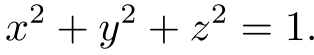
\includegraphics[width=88.23pt]{images-full/p268-i000.png}}\allowbreak{}.


% SOURCE_PDF_PAGE 269

\hypertarget{source-p269}{}
\sourceblock{432.79}{images-full/p269-d000.png}
直线\allowbreak{}\raisebox{-2.88pt}{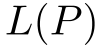
\includegraphics[width=28.81pt]{images-full/p269-i000.png}}\allowbreak{} 和过$Q$ 点的直线\allowbreak{}\raisebox{-2.88pt}{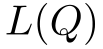
\includegraphics[width=28.81pt]{images-full/p269-i002.png}}\allowbreak{} 正交于点\allowbreak{}\raisebox{-2.16pt}{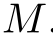
\includegraphics[width=14.74pt]{images-full/p269-i003.png}}\allowbreak{}问:所有可能的正交点$M$ 构成何种曲
面?证明你的结论.
解这是一个球面，兹证明如下.在空间中建立直角坐标系，使得线段\allowbreak{}\raisebox{-2.76pt}{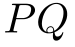
\includegraphics[width=20.90pt]{images-full/p269-i005.png}}\allowbreak{} 的中点为
原点\allowbreak{}\raisebox{-2.76pt}{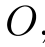
\includegraphics[width=12.37pt]{images-full/p269-i006.png}}\allowbreak{}，直线\allowbreak{}\raisebox{-2.88pt}{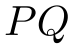
\includegraphics[width=20.90pt]{images-full/p269-i007.png}}\allowbreak{} 为$z$ 轴，
\sourceblock{175.15}{images-full/p269-d001.png}
设过$P$ 点的直线\allowbreak{}\raisebox{-2.88pt}{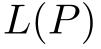
\includegraphics[width=28.25pt]{images-full/p269-i010.png}}\allowbreak{} 和过$Q$ 点的直线\allowbreak{}\raisebox{-2.88pt}{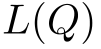
\includegraphics[width=28.25pt]{images-full/p269-i012.png}}\allowbreak{} 正交于\allowbreak{}\raisebox{-2.88pt}{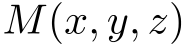
\includegraphics[width=53.11pt]{images-full/p269-i013.png}}\allowbreak{} 点，则有
\sourceblock{80.23}{images-full/p269-d002.png}
于是有
\sourceblock{154.24}{images-full/p269-d003.png}
\sourceblock{274.59}{images-full/p269-d004.png}
\par\medskip\noindent\textbf{【例6.2.2 】(第十三届全国初赛补赛题)设$S$ 为三维欧氏空间中的一个椭球面.$P$}
为空间中的一个固定点，$P$ 不在$S$ 上.对任意的\allowbreak{}\raisebox{-2.64pt}{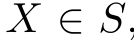
\includegraphics[width=37.43pt]{images-full/p269-i018.png}}\allowbreak{}，记\allowbreak{}\raisebox{-2.40pt}{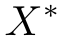
\includegraphics[width=17.51pt]{images-full/p269-i019.png}}\allowbreak{} 是线段\allowbreak{}\raisebox{-2.28pt}{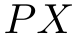
\includegraphics[width=22.03pt]{images-full/p269-i020.png}}\allowbreak{} 的中点.问:
所有这样的点\allowbreak{}\raisebox{-2.28pt}{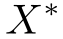
\includegraphics[width=17.51pt]{images-full/p269-i021.png}}\allowbreak{} 构成的轨迹是什么?证明你的结论.
\sourceblock{398.89}{images-full/p269-d005.png}
设固定点\allowbreak{}\raisebox{-3.00pt}{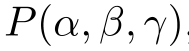
\includegraphics[width=53.29pt]{images-full/p269-i022.png}}\allowbreak{}，对于任意的\allowbreak{}\raisebox{-3.00pt}{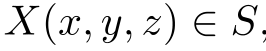
\includegraphics[width=74.83pt]{images-full/p269-i023.png}}\allowbreak{}，由题意有
\sourceblock{89.83}{images-full/p269-d006.png}
其中\allowbreak{}\raisebox{-3.00pt}{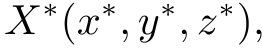
\includegraphics[width=73.65pt]{images-full/p269-i024.png}}\allowbreak{}则
\sourceblock{259.90}{images-full/p269-d007.png}


% SOURCE_PDF_PAGE 270

\hypertarget{source-p270}{}
\sourceblock{339.56}{images-full/p270-d000.png}
因为$X$在$S$上，所以有
\sourceblock{224.30}{images-full/p270-d001.png}
\sourceblock{355.95}{images-full/p270-d002.png}
\sourceblock{376.85}{images-full/p270-d003.png}
\sourceblock{183.06}{images-full/p270-d004.png}
及$S$外部一点\allowbreak{}\raisebox{-3.00pt}{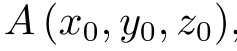
\includegraphics[width=66.51pt]{images-full/p270-i003.png}}\allowbreak{}，过$A$ 点且与$S$相切的所有直线构成锥面\allowbreak{}\raisebox{-2.28pt}{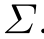
\includegraphics[width=12.27pt]{images-full/p270-i006.png}}\allowbreak{} 证明:存在平
面\allowbreak{}\raisebox{-2.04pt}{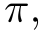
\includegraphics[width=10.89pt]{images-full/p270-i007.png}}\allowbreak{}，使得交线\allowbreak{}\raisebox{-2.76pt}{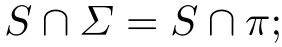
\includegraphics[width=79.43pt]{images-full/p270-i008.png}}\allowbreak{} 并求出平面\allowbreak{}\raisebox{-1.68pt}{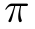
\includegraphics[width=9.60pt]{images-full/p270-i009.png}}\allowbreak{}的方程.
解(方法1) 因$A$ 在$S$ 的外部，故有
\sourceblock{287.02}{images-full/p270-d005.png}
对于任意的\allowbreak{}\raisebox{-3.00pt}{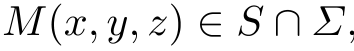
\includegraphics[width=99.67pt]{images-full/p270-i012.png}}\allowbreak{}，连接\allowbreak{}\raisebox{-2.64pt}{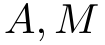
\includegraphics[width=29.38pt]{images-full/p270-i013.png}}\allowbreak{} 的直线记为\allowbreak{}\raisebox{-2.64pt}{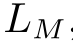
\includegraphics[width=20.29pt]{images-full/p270-i014.png}}\allowbreak{}，其参数方程可设为
\sourceblock{335.04}{images-full/p270-d006.png}
代入椭球面方程得
\sourceblock{311.31}{images-full/p270-d007.png}
\sourceblock{390.98}{images-full/p270-d008.png}


% SOURCE_PDF_PAGE 271

\hypertarget{source-p271}{}
\sourceblock{257.64}{images-full/p271-d000.png}
\sourceblock{315.27}{images-full/p271-d001.png}
\sourceblock{352.56}{images-full/p271-d002.png}
由于\allowbreak{}\raisebox{-2.64pt}{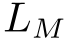
\includegraphics[width=19.21pt]{images-full/p271-i000.png}}\allowbreak{} 与$S$在$M$ 点相切，方程(6.2.3) 有一个二重根\allowbreak{}\raisebox{-2.64pt}{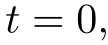
\includegraphics[width=30.46pt]{images-full/p271-i003.png}}\allowbreak{}故有
\sourceblock{296.06}{images-full/p271-d003.png}
此时由(6立1) 可知，方程(6.2.3) 的首项系数化为
\sourceblock{287.02}{images-full/p271-d004.png}
特别地，(6.2.4)的系数均不为霉，因而是一个平面方程，确定的平面记为\allowbreak{}\raisebox{-1.68pt}{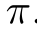
\includegraphics[width=10.10pt]{images-full/p271-i004.png}}\allowbreak{}.上述的推导
\par\noindent\textbf{证明}\ 了\allowbreak{}\raisebox{-2.76pt}{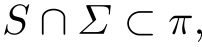
\includegraphics[width=56.79pt]{images-full/p271-i005.png}}\allowbreak{}，从而证明了\allowbreak{}\raisebox{-2.40pt}{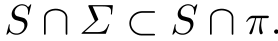
\includegraphics[width=78.25pt]{images-full/p271-i006.png}}\allowbreak{}
\sourceblock{433.35}{images-full/p271-d005.png}
两点确定的直线\allowbreak{}\raisebox{-2.64pt}{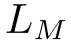
\includegraphics[width=19.77pt]{images-full/p271-i007.png}}\allowbreak{}一定在点$M$ 与$S$ 相切.故由定义，\allowbreak{}\raisebox{-2.64pt}{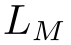
\includegraphics[width=19.77pt]{images-full/p271-i010.png}}\allowbreak{} 在锥面$E$ 上.特别地，
\allowbreak{}\raisebox{-2.64pt}{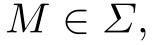
\includegraphics[width=42.79pt]{images-full/p271-i012.png}}\allowbreak{}由$M$ 的任意性，\allowbreak{}\raisebox{-2.40pt}{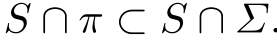
\includegraphics[width=77.99pt]{images-full/p271-i014.png}}\allowbreak{}
(方法2) 困$A$在$S$ 的外部，故有
\sourceblock{97.74}{images-full/p271-d006.png}
\sourceblock{429.40}{images-full/p271-d007.png}
\sourceblock{324.87}{images-full/p271-d008.png}


% SOURCE_PDF_PAGE 272

\hypertarget{source-p272}{}
\sourceblock{295.49}{images-full/p272-d000.png}
通过点\allowbreak{}\raisebox{-3.00pt}{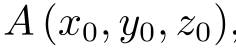
\includegraphics[width=66.39pt]{images-full/p272-i000.png}}\allowbreak{}，因而\allowbreak{}\raisebox{-2.64pt}{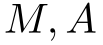
\includegraphics[width=28.81pt]{images-full/p272-i001.png}}\allowbreak{} 的连线在点$M$ 和椭球面$S$ 相切，它在锥面$E$，故\allowbreak{}\raisebox{-2.40pt}{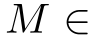
\includegraphics[width=26.55pt]{images-full/p272-i005.png}}\allowbreak{}
\allowbreak{}\raisebox{-2.28pt}{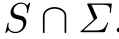
\includegraphics[width=33.29pt]{images-full/p272-i006.png}}\allowbreak{} 结论得证.
团组型玉树、刷、州时
1.柱面
由一族平行的直线构成的曲面称为柱面，这些直线称为直母线.柱面上的一条曲线如
果与所有的直母线都相交，就称它为柱面的一条准线.
柱面由直母线与准线确定.设\allowbreak{}\raisebox{-3.00pt}{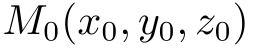
\includegraphics[width=71.19pt]{images-full/p272-i007.png}}\allowbreak{} 为准线
\sourceblock{287.58}{images-full/p272-d001.png}
\allowbreak{}\raisebox{-3.96pt}{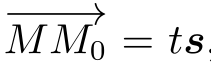
\includegraphics[width=59.15pt]{images-full/p272-i010.png}}\allowbreak{}
上的点，则对于经过\allowbreak{}\raisebox{-2.64pt}{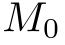
\includegraphics[width=18.08pt]{images-full/p272-i008.png}}\allowbreak{} 点的直母线上任意一点\allowbreak{}\raisebox{-3.00pt}{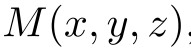
\includegraphics[width=53.44pt]{images-full/p272-i009.png}}\allowbreak{}，满足，其中$s$ 是
直母线的方向向量.因为\allowbreak{}\raisebox{-2.76pt}{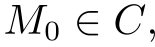
\includegraphics[width=43.46pt]{images-full/p272-i012.png}}\allowbreak{}，所以有
\sourceblock{326.57}{images-full/p272-d002.png}
消去参数$t$就可以获得柱面的方程.
\par\medskip\noindent\textbf{【例6.2.4】(第十五届全国初赛题)在空间中给定直线$L$ 以及直线外定点\allowbreak{}\raisebox{-2.16pt}{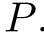
\includegraphics[width=12.20pt]{images-full/p272-i015.png}}\allowbreak{} 设$M$}
是过点$P$ 且与直线$L$ 相切的球面的球心.问:所有可能的球心$M$ 构成何种曲面7 证明
你的结论.
解所有可能的球心$M$ 构成抛物柱面，兹证明如下.在空间中建立直角坐标系，使
得直线$L$为$z$轴，点$P$ 到$L$ 的垂线为$z$轴，其垂足\allowbreak{}\raisebox{-2.40pt}{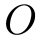
\includegraphics[width=11.86pt]{images-full/p272-i026.png}}\allowbreak{}为原点. 此时，设\allowbreak{}\raisebox{-3.00pt}{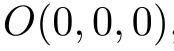
\includegraphics[width=48.82pt]{images-full/p272-i027.png}}\allowbreak{}，\allowbreak{}\raisebox{-3.00pt}{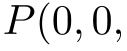
\includegraphics[width=35.51pt]{images-full/p272-i028.png}}\allowbreak{}
\allowbreak{}\raisebox{-2.88pt}{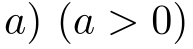
\includegraphics[width=54.24pt]{images-full/p272-i029.png}}\allowbreak{}，直线$L$ 的方向向量为\allowbreak{}\raisebox{-2.88pt}{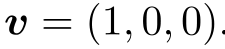
\includegraphics[width=63.23pt]{images-full/p272-i031.png}}\allowbreak{}. 设\allowbreak{}\raisebox{-2.88pt}{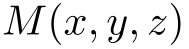
\includegraphics[width=53.11pt]{images-full/p272-i032.png}}\allowbreak{} 是过$P$ 点且与直线$L$ 相切
的球面的球心，则球半径\allowbreak{}\raisebox{-2.28pt}{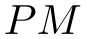
\includegraphics[width=24.29pt]{images-full/p272-i035.png}}\allowbreak{} 等于$M$ 到直线$L$ 的距离，即
\sourceblock{96.05}{images-full/p272-d003.png}
\sourceblock{302.84}{images-full/p272-d004.png}
\sourceblock{336.74}{images-full/p272-d005.png}


% SOURCE_PDF_PAGE 273

\hypertarget{source-p273}{}
可得
\sourceblock{151.42}{images-full/p273-d000.png}
\sourceblock{272.33}{images-full/p273-d001.png}
它是一个抛物柱面.
\par\medskip\noindent\textbf{【例6.2.51设柱面的准线方程为}
\sourceblock{137.86}{images-full/p273-d002.png}
母线的方向向量为\allowbreak{}\raisebox{-3.00pt}{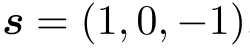
\includegraphics[width=70.57pt]{images-full/p273-i000.png}}\allowbreak{} 求柱面的方程.
解设\allowbreak{}\raisebox{-2.88pt}{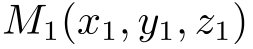
\includegraphics[width=71.19pt]{images-full/p273-i001.png}}\allowbreak{} 为准线$C$上任意一点，\allowbreak{}\raisebox{-2.88pt}{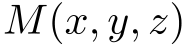
\includegraphics[width=53.11pt]{images-full/p273-i003.png}}\allowbreak{} 为连接\allowbreak{}\raisebox{-2.64pt}{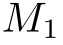
\includegraphics[width=17.51pt]{images-full/p273-i004.png}}\allowbreak{} 的母线上的任意
一点，则有
\sourceblock{303.97}{images-full/p273-d003.png}
\sourceblock{450.00}{images-full/p273-d004.png}
\sourceblock{106.22}{images-full/p273-d005.png}
即
\sourceblock{141.25}{images-full/p273-d006.png}
为所求柱面.
\sourceblock{450.00}{images-full/p273-d007.png}


% SOURCE_PDF_PAGE 274

\hypertarget{source-p274}{}
\allowbreak{}\raisebox{-3.00pt}{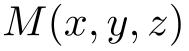
\includegraphics[width=53.11pt]{images-full/p274-i000.png}}\allowbreak{} 到母线的距离为困的半径.我们有
\sourceblock{236.73}{images-full/p274-d000.png}
因为
\sourceblock{213.00}{images-full/p274-d001.png}
\sourceblock{407.36}{images-full/p274-d002.png}
\sourceblock{447.48}{images-full/p274-d003.png}
\sourceblock{86.44}{images-full/p274-d004.png}
\sourceblock{285.32}{images-full/p274-d005.png}
设\allowbreak{}\raisebox{-3.00pt}{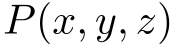
\includegraphics[width=49.72pt]{images-full/p274-i001.png}}\allowbreak{} 为圆柱面准线上任意一点，则有
\sourceblock{106.78}{images-full/p274-d006.png}
\sourceblock{315.83}{images-full/p274-d007.png}
(方法2) 过\allowbreak{}\raisebox{-3.00pt}{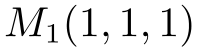
\includegraphics[width=55.93pt]{images-full/p274-i002.png}}\allowbreak{} 且与\allowbreak{}\raisebox{-2.52pt}{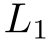
\includegraphics[width=14.12pt]{images-full/p274-i003.png}}\allowbreak{}垂直的平面\allowbreak{}\raisebox{-1.56pt}{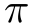
\includegraphics[width=9.60pt]{images-full/p274-i004.png}}\allowbreak{}为
\sourceblock{75.14}{images-full/p274-d008.png}


% SOURCE_PDF_PAGE 275

\hypertarget{source-p275}{}
经计算可得，平面\allowbreak{}\raisebox{-1.56pt}{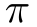
\includegraphics[width=10.17pt]{images-full/p275-i000.png}}\allowbreak{}与\allowbreak{}\raisebox{-2.52pt}{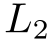
\includegraphics[width=15.25pt]{images-full/p275-i001.png}}\allowbreak{} 的交点为\allowbreak{}\raisebox{-3.00pt}{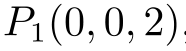
\includegraphics[width=52.26pt]{images-full/p275-i002.png}}\allowbreak{}，平面\allowbreak{}\raisebox{-1.56pt}{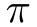
\includegraphics[width=10.17pt]{images-full/p275-i003.png}}\allowbreak{} 与\allowbreak{}\raisebox{-2.64pt}{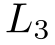
\includegraphics[width=15.25pt]{images-full/p275-i004.png}}\allowbreak{} 的交点为\allowbreak{}\raisebox{-3.00pt}{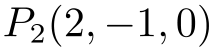
\includegraphics[width=61.02pt]{images-full/p275-i005.png}}\allowbreak{}. 可
以验证，\allowbreak{}\raisebox{-3.00pt}{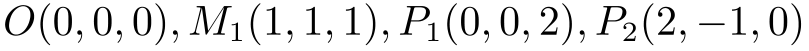
\includegraphics[width=228.26pt]{images-full/p275-i006.png}}\allowbreak{} 不共面，所以这四点可以确定一个
球面\allowbreak{}\raisebox{-2.28pt}{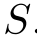
\includegraphics[width=10.06pt]{images-full/p275-i007.png}}\allowbreak{} 设$S$ 的方程满足
\sourceblock{181.36}{images-full/p275-d000.png}
将上述各点分别代入，可求得\allowbreak{}\raisebox{-2.76pt}{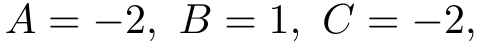
\includegraphics[width=134.47pt]{images-full/p275-i009.png}}\allowbreak{}，所以$S$ 的方程满足
\sourceblock{164.41}{images-full/p275-d001.png}
于是，圆柱面的准线方程为
\sourceblock{173.45}{images-full/p275-d002.png}
设\allowbreak{}\raisebox{-3.00pt}{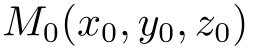
\includegraphics[width=71.19pt]{images-full/p275-i011.png}}\allowbreak{} 为圆柱面准线上任意一点，则过\allowbreak{}\raisebox{-3.00pt}{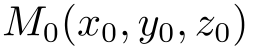
\includegraphics[width=71.19pt]{images-full/p275-i012.png}}\allowbreak{} 的母线\allowbreak{}\raisebox{-2.64pt}{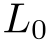
\includegraphics[width=14.69pt]{images-full/p275-i013.png}}\allowbreak{} 的方程为
\sourceblock{140.12}{images-full/p275-d003.png}
而\allowbreak{}\raisebox{-2.88pt}{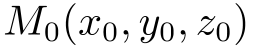
\includegraphics[width=71.19pt]{images-full/p275-i014.png}}\allowbreak{} 在准线上，则
\sourceblock{188.14}{images-full/p275-d004.png}
\sourceblock{316.40}{images-full/p275-d005.png}
2. 锥面
称一族经过一个固定点\allowbreak{}\raisebox{-2.64pt}{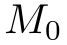
\includegraphics[width=18.64pt]{images-full/p275-i015.png}}\allowbreak{} 的直线构成的曲面为锥面.称这些直线为锥面的直母线，
\allowbreak{}\raisebox{-2.64pt}{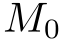
\includegraphics[width=18.08pt]{images-full/p275-i016.png}}\allowbreak{}为锥面的顶点锥面上不经过顶点的一条曲线如果和每一条直母线都相交，则称它为
锥面的一条准线.
设\allowbreak{}\raisebox{-3.00pt}{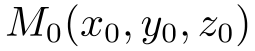
\includegraphics[width=71.75pt]{images-full/p275-i017.png}}\allowbreak{} 为锥面的顶点，\allowbreak{}\raisebox{-3.00pt}{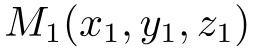
\includegraphics[width=71.75pt]{images-full/p275-i018.png}}\allowbreak{} 是准线
\sourceblock{287.58}{images-full/p275-d006.png}
\sourceblock{450.00}{images-full/p275-d007.png}
及\allowbreak{}\raisebox{-2.76pt}{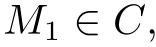
\includegraphics[width=44.00pt]{images-full/p275-i019.png}}\allowbreak{}，则有
\sourceblock{404.54}{images-full/p275-d008.png}
由上述方程组消去参数$t$ 即可获得锥面方程.


% SOURCE_PDF_PAGE 276

\hypertarget{source-p276}{}
\par\medskip\noindent\textbf{【例6.2.7】求顶点为原点\allowbreak{}\raisebox{-3.00pt}{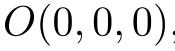
\includegraphics[width=49.20pt]{images-full/p276-i000.png}}\allowbreak{}，准线为}
\sourceblock{113.56}{images-full/p276-d000.png}
的锥面方程.
解设\allowbreak{}\raisebox{-2.88pt}{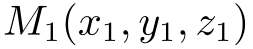
\includegraphics[width=71.19pt]{images-full/p276-i001.png}}\allowbreak{}为准线$C$上的任意一点，\allowbreak{}\raisebox{-3.00pt}{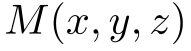
\includegraphics[width=53.67pt]{images-full/p276-i003.png}}\allowbreak{} 为连接顶点\allowbreak{}\raisebox{-2.40pt}{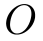
\includegraphics[width=11.86pt]{images-full/p276-i004.png}}\allowbreak{} 与\allowbreak{}\raisebox{-2.64pt}{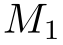
\includegraphics[width=17.51pt]{images-full/p276-i005.png}}\allowbreak{} 的
\sourceblock{450.00}{images-full/p276-d001.png}
\sourceblock{450.00}{images-full/p276-d002.png}
\sourceblock{96.61}{images-full/p276-d003.png}
\par\medskip\noindent\textbf{【例6.2.8] (第十三届全国初赛题)设球面\allowbreak{}\raisebox{-3.24pt}{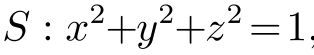
\includegraphics[width=88.48pt]{images-full/p276-i006.png}}\allowbreak{}，求以点\allowbreak{}\raisebox{-2.88pt}{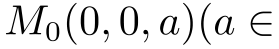
\includegraphics[width=78.53pt]{images-full/p276-i007.png}}\allowbreak{}}
\allowbreak{}\raisebox{-3.00pt}{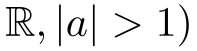
\includegraphics[width=55.37pt]{images-full/p276-i008.png}}\allowbreak{} 为顶点且与$S$ 相切的锥面方程.
解(方法1) 设$L$为过顶点\allowbreak{}\raisebox{-3.00pt}{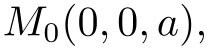
\includegraphics[width=58.41pt]{images-full/p276-i011.png}}\allowbreak{}，方向为\allowbreak{}\raisebox{-3.00pt}{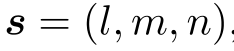
\includegraphics[width=65.76pt]{images-full/p276-i012.png}}\allowbreak{}，与$S$相切的锥面上的
任意一条母线，则对于$L$上任意一点\allowbreak{}\raisebox{-3.00pt}{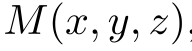
\includegraphics[width=54.15pt]{images-full/p276-i015.png}}\allowbreak{}，$L$ 的方程可以表示为
\sourceblock{124.86}{images-full/p276-d004.png}
其中\allowbreak{}\raisebox{-2.64pt}{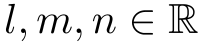
\includegraphics[width=57.63pt]{images-full/p276-i017.png}}\allowbreak{} 不全为零.设$L$ 的参数方程为
\sourceblock{74.58}{images-full/p276-d005.png}
其中\allowbreak{}\raisebox{-2.40pt}{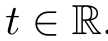
\includegraphics[width=30.28pt]{images-full/p276-i019.png}}\allowbreak{}R.将直线的参数方程代入$S$ 中可得
\sourceblock{197.75}{images-full/p276-d006.png}
由直线$L$与球面$S$相切的条件可知
\sourceblock{203.40}{images-full/p276-d007.png}


% SOURCE_PDF_PAGE 277

\hypertarget{source-p277}{}
\sourceblock{309.05}{images-full/p277-d000.png}
消去参数$t$可得锥面方程
\sourceblock{174.58}{images-full/p277-d001.png}
其中\allowbreak{}\raisebox{-3.00pt}{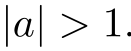
\includegraphics[width=36.72pt]{images-full/p277-i001.png}}\allowbreak{}.
(方法2) 设0(0 ，0 ，0) 为球心坐标，M怡，y ，z) 为切锥面与球面的切点，半顶角为
\sourceblock{245.77}{images-full/p277-d002.png}
\sourceblock{251.42}{images-full/p277-d003.png}
\sourceblock{303.97}{images-full/p277-d004.png}
即
\sourceblock{174.58}{images-full/p277-d005.png}
其中\allowbreak{}\raisebox{-3.00pt}{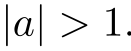
\includegraphics[width=36.72pt]{images-full/p277-i002.png}}\allowbreak{}.
3. 旋转曲面
空间一条曲线$C$绕某条直线$l$旋转而得到的由面称为旋转曲面，称\allowbreak{}\raisebox{-2.28pt}{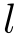
\includegraphics[width=6.21pt]{images-full/p277-i005.png}}\allowbreak{}为它的轴线，$C$
为它的母线.
设轴线$l$经过\allowbreak{}\raisebox{-3.00pt}{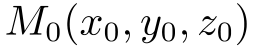
\includegraphics[width=71.75pt]{images-full/p277-i008.png}}\allowbreak{} 点，方向为\allowbreak{}\raisebox{-1.68pt}{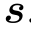
\includegraphics[width=8.69pt]{images-full/p277-i009.png}}\allowbreak{} 设\allowbreak{}\raisebox{-3.00pt}{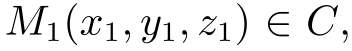
\includegraphics[width=99.32pt]{images-full/p277-i010.png}}\allowbreak{}则$C$ 绕$l$旋转经
过\allowbreak{}\raisebox{-2.64pt}{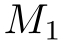
\includegraphics[width=18.08pt]{images-full/p277-i013.png}}\allowbreak{} 的纬圆所在的平面与$l$垂直.再设\allowbreak{}\raisebox{-3.00pt}{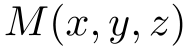
\includegraphics[width=53.67pt]{images-full/p277-i015.png}}\allowbreak{} 为旋转曲面上任意一点，则旋转曲
\sourceblock{450.00}{images-full/p277-d006.png}
\sourceblock{292.10}{images-full/p277-d007.png}
旋转所得的旋转曲面方程.


% SOURCE_PDF_PAGE 278

\hypertarget{source-p278}{}
解设\allowbreak{}\raisebox{-3.00pt}{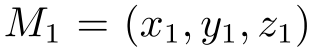
\includegraphics[width=88.70pt]{images-full/p278-i000.png}}\allowbreak{} 为\allowbreak{}\raisebox{-2.52pt}{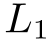
\includegraphics[width=14.12pt]{images-full/p278-i001.png}}\allowbreak{}上任意一点，\allowbreak{}\raisebox{-2.88pt}{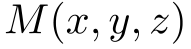
\includegraphics[width=53.67pt]{images-full/p278-i002.png}}\allowbreak{} 为过\allowbreak{}\raisebox{-2.52pt}{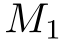
\includegraphics[width=17.51pt]{images-full/p278-i003.png}}\allowbreak{} 绕\allowbreak{}\raisebox{-2.52pt}{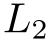
\includegraphics[width=14.69pt]{images-full/p278-i004.png}}\allowbreak{}旋转的纬圆
上任意一点，\allowbreak{}\raisebox{-3.00pt}{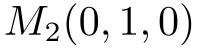
\includegraphics[width=55.93pt]{images-full/p278-i005.png}}\allowbreak{} 为\allowbreak{}\raisebox{-2.64pt}{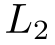
\includegraphics[width=15.25pt]{images-full/p278-i006.png}}\allowbreak{}上的点\allowbreak{}\raisebox{-3.00pt}{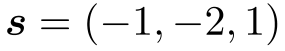
\includegraphics[width=80.23pt]{images-full/p278-i007.png}}\allowbreak{} 为\allowbreak{}\raisebox{-2.64pt}{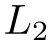
\includegraphics[width=14.69pt]{images-full/p278-i008.png}}\allowbreak{} 的方向向量.于是有
\sourceblock{333.35}{images-full/p278-d000.png}
\sourceblock{163.28}{images-full/p278-d001.png}
于是可得
\sourceblock{333.91}{images-full/p278-d002.png}
\sourceblock{339.56}{images-full/p278-d003.png}
为所求的旋转曲面.
\par\medskip\noindent\textbf{【例6.2.10】(第十一届全国初赛题)空间中有两个球面\allowbreak{}\raisebox{-2.64pt}{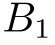
\includegraphics[width=15.25pt]{images-full/p278-i009.png}}\allowbreak{}和\allowbreak{}\raisebox{-2.64pt}{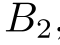
\includegraphics[width=16.51pt]{images-full/p278-i010.png}}\allowbreak{} 且\allowbreak{}\raisebox{-2.64pt}{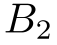
\includegraphics[width=15.82pt]{images-full/p278-i011.png}}\allowbreak{}包含在\allowbreak{}\raisebox{-2.64pt}{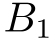
\includegraphics[width=15.25pt]{images-full/p278-i012.png}}\allowbreak{}}
所围球体的内部，两个球面之间的闭区域为\allowbreak{}\raisebox{-2.28pt}{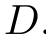
\includegraphics[width=12.65pt]{images-full/p278-i013.png}}\allowbreak{} 设$B$ 是含在$D$ 中的一个圆球，它与球面
\allowbreak{}\raisebox{-2.64pt}{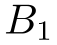
\includegraphics[width=15.82pt]{images-full/p278-i016.png}}\allowbreak{}和\allowbreak{}\raisebox{-2.64pt}{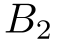
\includegraphics[width=16.38pt]{images-full/p278-i017.png}}\allowbreak{}均相切.问:
\par\noindent (1) $B$ 的球心轨迹构成的曲面$S$是何种曲面?
\par\noindent (2) \allowbreak{}\raisebox{-2.64pt}{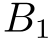
\includegraphics[width=15.25pt]{images-full/p278-i020.png}}\allowbreak{}的球心和\allowbreak{}\raisebox{-2.64pt}{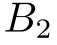
\includegraphics[width=15.82pt]{images-full/p278-i021.png}}\allowbreak{} 的球心是曲面$S$ 的何种点?
\par\noindent\textbf{证明}\ 你的论断.
解结论: (1) $B$ 的球心轨迹构成的曲面$S$ 为旋转椭球面j (2) \allowbreak{}\raisebox{-2.64pt}{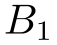
\includegraphics[width=15.82pt]{images-full/p278-i025.png}}\allowbreak{}和\allowbreak{}\raisebox{-2.64pt}{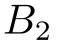
\includegraphics[width=15.82pt]{images-full/p278-i026.png}}\allowbreak{}的球心为$S$
的两个焦点证明如下.
设\allowbreak{}\raisebox{-2.64pt}{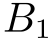
\includegraphics[width=15.25pt]{images-full/p278-i028.png}}\allowbreak{} 的球心为\allowbreak{}\raisebox{-2.76pt}{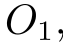
\includegraphics[width=17.64pt]{images-full/p278-i029.png}}\allowbreak{}半径为\allowbreak{}\raisebox{-2.64pt}{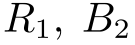
\includegraphics[width=37.85pt]{images-full/p278-i030.png}}\allowbreak{} 的球心为\allowbreak{}\raisebox{-2.76pt}{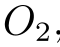
\includegraphics[width=16.55pt]{images-full/p278-i031.png}}\allowbreak{}，半径为\allowbreak{}\raisebox{-2.64pt}{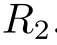
\includegraphics[width=15.78pt]{images-full/p278-i032.png}}\allowbreak{}.设$B$ 是含在$D$ 中
的一个球，球心在$P$ 点，半径为$r$，它与球\allowbreak{}\raisebox{-2.64pt}{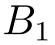
\includegraphics[width=15.25pt]{images-full/p278-i037.png}}\allowbreak{} 和\allowbreak{}\raisebox{-2.64pt}{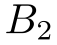
\includegraphics[width=15.82pt]{images-full/p278-i038.png}}\allowbreak{} 均相切.因为$B$ 与\allowbreak{}\raisebox{-2.64pt}{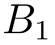
\includegraphics[width=15.25pt]{images-full/p278-i040.png}}\allowbreak{} 内切，所以


% SOURCE_PDF_PAGE 279

\hypertarget{source-p279}{}
\allowbreak{}\raisebox{-2.64pt}{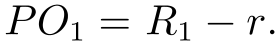
\includegraphics[width=77.27pt]{images-full/p279-i000.png}}\allowbreak{} 因为$B$ 与\allowbreak{}\raisebox{-2.52pt}{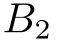
\includegraphics[width=15.82pt]{images-full/p279-i002.png}}\allowbreak{} 外切，所以\allowbreak{}\raisebox{-2.64pt}{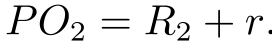
\includegraphics[width=76.66pt]{images-full/p279-i003.png}}\allowbreak{} 于是有
\sourceblock{121.47}{images-full/p279-d000.png}
为常数.
设$L$是过球心\allowbreak{}\raisebox{-2.64pt}{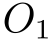
\includegraphics[width=15.25pt]{images-full/p279-i005.png}}\allowbreak{}和\allowbreak{}\raisebox{-2.64pt}{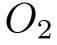
\includegraphics[width=15.82pt]{images-full/p279-i006.png}}\allowbreak{} 的直线.困\allowbreak{}\raisebox{-2.64pt}{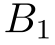
\includegraphics[width=15.25pt]{images-full/p279-i007.png}}\allowbreak{}和\allowbreak{}\raisebox{-2.64pt}{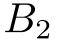
\includegraphics[width=15.82pt]{images-full/p279-i008.png}}\allowbreak{} 在以$L$为不动轴的空间旋转下不变，
故区域$D$ 也在以$L$为不动轴的空间旋转下不变.$B$ 在以$L$ 为不动轴的空间旋转下保持
\sourceblock{450.00}{images-full/p279-d001.png}
一个椭圆，故B 的球心轨迹构成的曲面$S$为旋转椭球面，旋转轴为过01 和O2 的直线，
且球心\allowbreak{}\raisebox{-2.76pt}{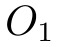
\includegraphics[width=15.82pt]{images-full/p279-i015.png}}\allowbreak{}和\allowbreak{}\raisebox{-2.76pt}{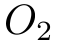
\includegraphics[width=16.38pt]{images-full/p279-i016.png}}\allowbreak{}为旋转椭球面的两个焦点
\sourceblock{245.77}{images-full/p279-d002.png}
绕$z$轴旋转所得的旋转曲面方程，并说明是什么曲面，其中\allowbreak{}\raisebox{-2.88pt}{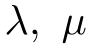
\includegraphics[width=25.99pt]{images-full/p279-i018.png}}\allowbreak{} 是常数.
\sourceblock{433.35}{images-full/p279-d003.png}
\allowbreak{}\raisebox{-3.00pt}{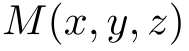
\includegraphics[width=53.11pt]{images-full/p279-i019.png}}\allowbreak{} 是过\allowbreak{}\raisebox{-2.64pt}{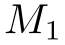
\includegraphics[width=18.08pt]{images-full/p279-i020.png}}\allowbreak{}绕$z$轴旋转的纬圆上任意一点于是有
\sourceblock{109.04}{images-full/p279-d004.png}
\sourceblock{300.01}{images-full/p279-d005.png}
由此可得\allowbreak{}\raisebox{-2.88pt}{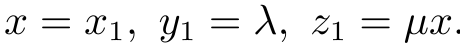
\includegraphics[width=129.62pt]{images-full/p279-i022.png}}\allowbreak{} 于是有
\sourceblock{244.64}{images-full/p279-d006.png}
\sourceblock{283.06}{images-full/p279-d007.png}
于是，当\allowbreak{}\raisebox{-2.76pt}{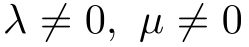
\includegraphics[width=70.06pt]{images-full/p279-i023.png}}\allowbreak{} 时，所得旋转曲面是单叶双曲面;当\allowbreak{}\raisebox{-2.76pt}{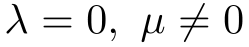
\includegraphics[width=70.06pt]{images-full/p279-i024.png}}\allowbreak{}时，所得旋转曲
面是圆锥面i 当\allowbreak{}\raisebox{-2.88pt}{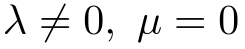
\includegraphics[width=68.93pt]{images-full/p279-i025.png}}\allowbreak{} 时，所得旋转曲面是圆柱面.
\par\medskip\noindent\textbf{【例6.2.12 】(第一届全国决赛题)己知两条直线的方程}
\sourceblock{216.96}{images-full/p279-d008.png}


% SOURCE_PDF_PAGE 280

\hypertarget{source-p280}{}
\par\noindent (1) 问:参数\allowbreak{}\raisebox{-2.76pt}{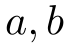
\includegraphics[width=19.77pt]{images-full/p280-i000.png}}\allowbreak{} 满足什么条件时，$L$与\allowbreak{}\raisebox{-2.40pt}{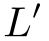
\includegraphics[width=13.56pt]{images-full/p280-i002.png}}\allowbreak{}是异面直线?
\par\noindent (2) 当$L$与\allowbreak{}\raisebox{-2.52pt}{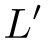
\includegraphics[width=13.56pt]{images-full/p280-i004.png}}\allowbreak{}不重合时，求\allowbreak{}\raisebox{-2.52pt}{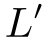
\includegraphics[width=13.56pt]{images-full/p280-i005.png}}\allowbreak{} 绕$L$旋转所生成的旋转曲面\allowbreak{}\raisebox{-1.56pt}{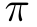
\includegraphics[width=10.17pt]{images-full/p280-i007.png}}\allowbreak{}的方程，并指出曲面
\allowbreak{}\raisebox{-1.68pt}{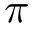
\includegraphics[width=9.60pt]{images-full/p280-i008.png}}\allowbreak{}的类型.
解(1) 易知直线\allowbreak{}\raisebox{-2.88pt}{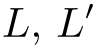
\includegraphics[width=28.25pt]{images-full/p280-i009.png}}\allowbreak{}的方向向量分别为
\sourceblock{145.20}{images-full/p280-d000.png}
分别取\allowbreak{}\raisebox{-3.00pt}{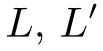
\includegraphics[width=28.81pt]{images-full/p280-i010.png}}\allowbreak{}上的点\allowbreak{}\raisebox{-3.00pt}{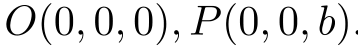
\includegraphics[width=100.90pt]{images-full/p280-i011.png}}\allowbreak{} 则$L$与\allowbreak{}\raisebox{-2.52pt}{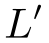
\includegraphics[width=13.56pt]{images-full/p280-i013.png}}\allowbreak{}是异面直线当且仅当向量\allowbreak{}\raisebox{-3.96pt}{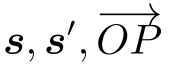
\includegraphics[width=47.46pt]{images-full/p280-i014.png}}\allowbreak{}
不共面，这等价于它们的混合积不为霉，即
\sourceblock{450.00}{images-full/p280-d001.png}
\sourceblock{315.27}{images-full/p280-d002.png}
\sourceblock{450.00}{images-full/p280-d003.png}
因为$L$经过坐标原点，所以点\allowbreak{}\raisebox{-2.88pt}{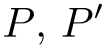
\includegraphics[width=31.07pt]{images-full/p280-i016.png}}\allowbreak{}与原点的距离相等，故
\sourceblock{306.23}{images-full/p280-d004.png}
\sourceblock{450.00}{images-full/p280-d005.png}
将(6.2.18) 式代入(6.2.15) 式，得
\sourceblock{292.10}{images-full/p280-d006.png}
当\allowbreak{}\raisebox{-2.76pt}{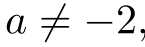
\includegraphics[width=40.63pt]{images-full/p280-i017.png}}\allowbreak{}，即$L$与\allowbreak{}\raisebox{-2.52pt}{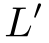
\includegraphics[width=13.56pt]{images-full/p280-i019.png}}\allowbreak{}不垂直时，解得
\sourceblock{131.64}{images-full/p280-d007.png}


% SOURCE_PDF_PAGE 281

\hypertarget{source-p281}{}
据此，再将(6.2.18) 式代入(6.2.17) 式，得到曲面\allowbreak{}\raisebox{-1.56pt}{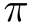
\includegraphics[width=9.60pt]{images-full/p281-i000.png}}\allowbreak{}的方程
\sourceblock{375.72}{images-full/p281-d000.png}
当\allowbreak{}\raisebox{-2.28pt}{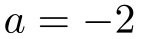
\includegraphics[width=39.55pt]{images-full/p281-i001.png}}\allowbreak{} 时，由(6.2.19) 式得\allowbreak{}\raisebox{-2.76pt}{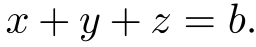
\includegraphics[width=71.92pt]{images-full/p281-i002.png}}\allowbreak{} 这表明\allowbreak{}\raisebox{-1.68pt}{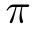
\includegraphics[width=10.17pt]{images-full/p281-i003.png}}\allowbreak{}在这个平面上.同时，将(6.2.18)
式代入(6.2.17) 式，有
\sourceblock{361.60}{images-full/p281-d001.png}
由于$t$的任意性，所以这时曲面\allowbreak{}\raisebox{-1.68pt}{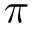
\includegraphics[width=9.60pt]{images-full/p281-i005.png}}\allowbreak{}的方程为
\sourceblock{112.43}{images-full/p281-d002.png}
曲面\allowbreak{}\raisebox{-1.56pt}{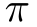
\includegraphics[width=10.17pt]{images-full/p281-i006.png}}\allowbreak{}的类型:当\allowbreak{}\raisebox{-2.28pt}{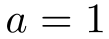
\includegraphics[width=30.51pt]{images-full/p281-i007.png}}\allowbreak{}且\allowbreak{}\raisebox{-2.76pt}{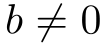
\includegraphics[width=29.94pt]{images-full/p281-i008.png}}\allowbreak{} 时，$L$与\allowbreak{}\raisebox{-2.40pt}{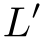
\includegraphics[width=12.99pt]{images-full/p281-i010.png}}\allowbreak{}平行，\allowbreak{}\raisebox{-1.56pt}{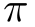
\includegraphics[width=9.60pt]{images-full/p281-i011.png}}\allowbreak{}为一柱面;当\allowbreak{}\raisebox{-2.88pt}{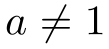
\includegraphics[width=30.51pt]{images-full/p281-i012.png}}\allowbreak{} 且\allowbreak{}\raisebox{-2.40pt}{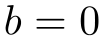
\includegraphics[width=29.94pt]{images-full/p281-i013.png}}\allowbreak{}
时，若\allowbreak{}\raisebox{-2.76pt}{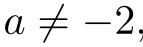
\includegraphics[width=39.98pt]{images-full/p281-i014.png}}\allowbreak{}，则$L$ 与\allowbreak{}\raisebox{-2.52pt}{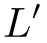
\includegraphics[width=12.99pt]{images-full/p281-i016.png}}\allowbreak{}相交，\allowbreak{}\raisebox{-1.56pt}{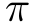
\includegraphics[width=9.60pt]{images-full/p281-i017.png}}\allowbreak{}为一锥面;若\allowbreak{}\raisebox{-2.64pt}{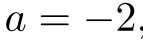
\includegraphics[width=40.10pt]{images-full/p281-i018.png}}\allowbreak{}，则\allowbreak{}\raisebox{-1.56pt}{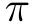
\includegraphics[width=9.60pt]{images-full/p281-i019.png}}\allowbreak{}是平面i 当\allowbreak{}\raisebox{-2.76pt}{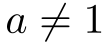
\includegraphics[width=30.51pt]{images-full/p281-i020.png}}\allowbreak{} 且\allowbreak{}\raisebox{-2.76pt}{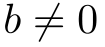
\includegraphics[width=29.38pt]{images-full/p281-i021.png}}\allowbreak{}
时，若\allowbreak{}\raisebox{-2.76pt}{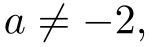
\includegraphics[width=41.74pt]{images-full/p281-i022.png}}\allowbreak{}，则\allowbreak{}\raisebox{-1.68pt}{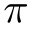
\includegraphics[width=9.60pt]{images-full/p281-i023.png}}\allowbreak{}为一单叶双曲面;若\allowbreak{}\raisebox{-2.64pt}{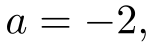
\includegraphics[width=42.94pt]{images-full/p281-i024.png}}\allowbreak{}，则\allowbreak{}\raisebox{-1.68pt}{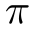
\includegraphics[width=9.60pt]{images-full/p281-i025.png}}\allowbreak{}为去掉一个圆盘后的平面.
\par\medskip\noindent\textbf{【例6.2.13】(第十三届全国初赛题)设不全为零的\allowbreak{}\raisebox{-2.64pt}{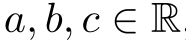
\includegraphics[width=52.29pt]{images-full/p281-i026.png}}\allowbreak{}，求直线}
\sourceblock{120.91}{images-full/p281-d003.png}
绕$z$轴旋转所得的旋转曲面方程.
解设点\allowbreak{}\raisebox{-3.00pt}{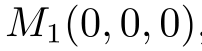
\includegraphics[width=56.82pt]{images-full/p281-i028.png}}\allowbreak{}，方向\allowbreak{}\raisebox{-3.00pt}{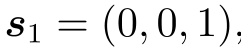
\includegraphics[width=67.58pt]{images-full/p281-i029.png}}\allowbreak{}，则$z$ 轴为直线
\sourceblock{90.96}{images-full/p281-d004.png}
\sourceblock{302.27}{images-full/p281-d005.png}
过\allowbreak{}\raisebox{-2.88pt}{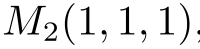
\includegraphics[width=56.10pt]{images-full/p281-i031.png}}\allowbreak{}，方向为\allowbreak{}\raisebox{-2.88pt}{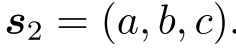
\includegraphics[width=66.47pt]{images-full/p281-i032.png}}\allowbreak{} 经计算可得混合积
\sourceblock{125.99}{images-full/p281-d006.png}
当\allowbreak{}\raisebox{-2.40pt}{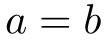
\includegraphics[width=30.51pt]{images-full/p281-i033.png}}\allowbreak{} 时，\allowbreak{}\raisebox{-2.52pt}{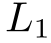
\includegraphics[width=14.12pt]{images-full/p281-i034.png}}\allowbreak{}与\allowbreak{}\raisebox{-2.52pt}{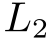
\includegraphics[width=14.69pt]{images-full/p281-i035.png}}\allowbreak{}共面.分三种情况讨论
\par\noindent (1) 当\allowbreak{}\raisebox{-2.64pt}{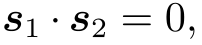
\includegraphics[width=56.75pt]{images-full/p281-i036.png}}\allowbreak{}，即\allowbreak{}\raisebox{-2.28pt}{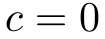
\includegraphics[width=29.38pt]{images-full/p281-i037.png}}\allowbreak{} 时，\allowbreak{}\raisebox{-2.64pt}{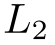
\includegraphics[width=15.25pt]{images-full/p281-i038.png}}\allowbreak{} 与\allowbreak{}\raisebox{-2.64pt}{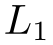
\includegraphics[width=14.69pt]{images-full/p281-i039.png}}\allowbreak{}垂直，此时所得的旋转曲面是$z=l$ 的平面.
\par\noindent (2) 当\allowbreak{}\raisebox{-2.76pt}{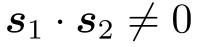
\includegraphics[width=55.93pt]{images-full/p281-i041.png}}\allowbreak{} 且\allowbreak{}\raisebox{-2.64pt}{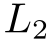
\includegraphics[width=15.25pt]{images-full/p281-i042.png}}\allowbreak{}平行于\allowbreak{}\raisebox{-2.64pt}{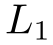
\includegraphics[width=14.69pt]{images-full/p281-i043.png}}\allowbreak{}时，所得旋转曲面是一个圆柱面\allowbreak{}\raisebox{-3.12pt}{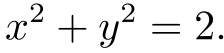
\includegraphics[width=63.05pt]{images-full/p281-i044.png}}\allowbreak{}
\sourceblock{450.00}{images-full/p281-d007.png}


% SOURCE_PDF_PAGE 282

\hypertarget{source-p282}{}
当\allowbreak{}\raisebox{-2.88pt}{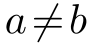
\includegraphics[width=25.99pt]{images-full/p282-i000.png}}\allowbreak{} 时，即\allowbreak{}\raisebox{-2.52pt}{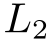
\includegraphics[width=15.25pt]{images-full/p282-i001.png}}\allowbreak{}与\allowbreak{}\raisebox{-2.52pt}{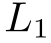
\includegraphics[width=14.12pt]{images-full/p282-i002.png}}\allowbreak{}不共面时，首先考虑\allowbreak{}\raisebox{-2.52pt}{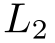
\includegraphics[width=15.25pt]{images-full/p282-i003.png}}\allowbreak{}与\allowbreak{}\raisebox{-2.52pt}{\includegraphics[width=14.12pt]{images-full/p282-i004.png}}\allowbreak{}不垂直的情形.设\allowbreak{}\raisebox{-2.88pt}{\includegraphics[width=71.75pt]{images-full/p282-i005.png}}\allowbreak{}
为\allowbreak{}\raisebox{-2.64pt}{\includegraphics[width=15.25pt]{images-full/p282-i006.png}}\allowbreak{}上任意一点，\allowbreak{}\raisebox{-3.00pt}{\includegraphics[width=53.11pt]{images-full/p282-i007.png}}\allowbreak{} 为过\allowbreak{}\raisebox{-2.64pt}{\includegraphics[width=18.64pt]{images-full/p282-i008.png}}\allowbreak{} 的旋转面上的纬圆上的任意一点，则有
\sourceblock{148.59}{images-full/p282-d000.png}
由此可得
\sourceblock{156.50}{images-full/p282-d001.png}
\sourceblock{446.91}{images-full/p282-d002.png}
\sourceblock{340.13}{images-full/p282-d003.png}
\sourceblock{404.54}{images-full/p282-d004.png}
\sourceblock{286.45}{images-full/p282-d005.png}
\sourceblock{351.43}{images-full/p282-d006.png}


% SOURCE_PDF_PAGE 283

\hypertarget{source-p283}{}
\sourceblock{450.00}{images-full/p283-d000.png}
\sourceblock{450.00}{images-full/p283-d001.png}
为\allowbreak{}\raisebox{-1.68pt}{\includegraphics[width=8.32pt]{images-full/p283-i000.png}}\allowbreak{} 设$B$是一个球心在$M$ 点的球，它与$S$外切并和\allowbreak{}\raisebox{-1.56pt}{\includegraphics[width=9.60pt]{images-full/p283-i004.png}}\allowbreak{}相切.
问:(1) 所有可能的$M$ 构成何种曲面?
\par\noindent (2) 点$P$与该曲面有何关系?证明你的结论.
解(几何法)过$P$作平面\allowbreak{}\raisebox{-1.56pt}{\includegraphics[width=9.60pt]{images-full/p283-i008.png}}\allowbreak{}的垂线，垂足为\allowbreak{}\raisebox{-2.40pt}{\includegraphics[width=11.82pt]{images-full/p283-i009.png}}\allowbreak{} 在垂线\allowbreak{}\raisebox{-2.40pt}{\includegraphics[width=20.90pt]{images-full/p283-i010.png}}\allowbreak{} 的延长线上取一点$Q$，
使得\allowbreak{}\raisebox{-3.00pt}{\includegraphics[width=50.59pt]{images-full/p283-i012.png}}\allowbreak{} 过$Q$ 点作平面\allowbreak{}\raisebox{-1.68pt}{\includegraphics[width=9.60pt]{images-full/p283-i014.png}}\allowbreak{}的平行平面\allowbreak{}\raisebox{-2.28pt}{\includegraphics[width=14.12pt]{images-full/p283-i015.png}}\allowbreak{}.这样两个平行平面付和\allowbreak{}\raisebox{-2.28pt}{\includegraphics[width=13.56pt]{images-full/p283-i017.png}}\allowbreak{}的距离为
\allowbreak{}\raisebox{-1.68pt}{\includegraphics[width=8.53pt]{images-full/p283-i018.png}}\allowbreak{} 于是，$M$ 到$P$ 的距离等于$M$ 到平面\allowbreak{}\raisebox{-2.40pt}{\includegraphics[width=13.56pt]{images-full/p283-i022.png}}\allowbreak{}的距离.于是，在过直线\allowbreak{}\raisebox{-2.76pt}{\includegraphics[width=21.36pt]{images-full/p283-i023.png}}\allowbreak{} 和$M$ 的平面\allowbreak{}\raisebox{-1.68pt}{\includegraphics[width=10.17pt]{images-full/p283-i025.png}}\allowbreak{}
上，$M$ 到点$P$ 的距离等于到交线\allowbreak{}\raisebox{-2.40pt}{\includegraphics[width=35.03pt]{images-full/p283-i028.png}}\allowbreak{}的距离，$M$ 的轨迹为抛物线，并以$P$ 为抛物线
的焦点以\allowbreak{}\raisebox{-2.76pt}{\includegraphics[width=20.90pt]{images-full/p283-i031.png}}\allowbreak{} 为轴作空间的旋转时，球$B$ 保持与球面$S$ 和平面\allowbreak{}\raisebox{-1.56pt}{\includegraphics[width=9.60pt]{images-full/p283-i034.png}}\allowbreak{}相切，$M$ 画出一个
圆周.故所有可能的$M$ 构成一个旋转抛物面，并以$P$ 为其焦点.
(坐标法)过$P$ 作平面\allowbreak{}\raisebox{-1.56pt}{\includegraphics[width=9.60pt]{images-full/p283-i039.png}}\allowbreak{}的垂线，垂足为\allowbreak{}\raisebox{-2.28pt}{\includegraphics[width=11.68pt]{images-full/p283-i040.png}}\allowbreak{} 以\allowbreak{}\raisebox{-2.28pt}{\includegraphics[width=11.86pt]{images-full/p283-i041.png}}\allowbreak{} 为原点，向量\allowbreak{}\raisebox{-3.48pt}{\includegraphics[width=21.47pt]{images-full/p283-i042.png}}\allowbreak{} 所在直线为$z$
轴，平面\allowbreak{}\raisebox{-1.68pt}{\includegraphics[width=9.60pt]{images-full/p283-i044.png}}\allowbreak{}为\allowbreak{}\raisebox{-2.76pt}{\includegraphics[width=25.42pt]{images-full/p283-i045.png}}\allowbreak{}平面，建立空间直角坐标系.设球$B$ 的球心$M$ 的坐标为\allowbreak{}\raisebox{-3.00pt}{\includegraphics[width=57.63pt]{images-full/p283-i048.png}}\allowbreak{}
点坐标为\allowbreak{}\raisebox{-2.88pt}{\includegraphics[width=43.49pt]{images-full/p283-i049.png}}\allowbreak{}，则有\allowbreak{}\raisebox{-3.00pt}{\includegraphics[width=72.51pt]{images-full/p283-i050.png}}\allowbreak{} 于是，有
\sourceblock{206.79}{images-full/p283-d002.png}
故所有的$M$ 构成一个旋转抛物面.因为标准的抛物面方程为
\sourceblock{122.60}{images-full/p283-d003.png}
\sourceblock{450.00}{images-full/p283-d004.png}
\sourceblock{210.74}{images-full/p283-d005.png}
于是，$P$ 点恰为旋转抛物面的焦点.
4. 坐标面上的曲线绕坐标轴旋转所得旋转曲面方程
设xOy 平面上的曲线
\sourceblock{281.93}{images-full/p283-d006.png}


% SOURCE_PDF_PAGE 284

\hypertarget{source-p284}{}
绕$z$轴、$u$ 轴旋转所得旋转面分别是\allowbreak{}\raisebox{-3.48pt}{\includegraphics[width=114.13pt]{images-full/p284-i002.png}}\allowbreak{} 以及\allowbreak{}\raisebox{-3.36pt}{\includegraphics[width=112.77pt]{images-full/p284-i003.png}}\allowbreak{}
类似地，可以获得其他坐标平面上的曲线绕坐标轴旋转所得的旋转曲面.
\sourceblock{324.87}{images-full/p284-d000.png}
\sourceblock{277.41}{images-full/p284-d001.png}
\sourceblock{396.06}{images-full/p284-d002.png}
\sourceblock{277.41}{images-full/p284-d003.png}
对于\allowbreak{}\raisebox{-2.76pt}{\includegraphics[width=25.42pt]{images-full/p284-i004.png}}\allowbreak{}平面上的抛物线\allowbreak{}\raisebox{-3.12pt}{\includegraphics[width=87.20pt]{images-full/p284-i005.png}}\allowbreak{}绕$z$ 轴旋转所得曲面为旋转抛物面
\sourceblock{76.27}{images-full/p284-d004.png}
\par\medskip\noindent\textbf{【例6.2.15 】(第十二届全国决赛题)给定\allowbreak{}\raisebox{-2.88pt}{\includegraphics[width=24.29pt]{images-full/p284-i007.png}}\allowbreak{}平面上的圆}
\sourceblock{246.90}{images-full/p284-d005.png}
\par\noindent (1) 求$C$绕$z$轴旋转所得到的环面$S$ 的隐式方程.
\par\noindent (2) 设\allowbreak{}\raisebox{-2.64pt}{\includegraphics[width=37.09pt]{images-full/p284-i011.png}}\allowbreak{}，以\allowbreak{}\raisebox{-3.00pt}{\includegraphics[width=58.76pt]{images-full/p284-i012.png}}\allowbreak{} 为顶点的两个锥面\allowbreak{}\raisebox{-2.64pt}{\includegraphics[width=13.56pt]{images-full/p284-i013.png}}\allowbreak{} 和\allowbreak{}\raisebox{-2.64pt}{\includegraphics[width=14.12pt]{images-full/p284-i014.png}}\allowbreak{}的半顶角之差为\allowbreak{}\raisebox{-3.00pt}{\includegraphics[width=22.02pt]{images-full/p284-i015.png}}\allowbreak{}，且
均与环面$S$ 相切(每条母线都与环面相切)，求\allowbreak{}\raisebox{-2.04pt}{\includegraphics[width=12.43pt]{images-full/p284-i017.png}}\allowbreak{}的值和品\allowbreak{}\raisebox{-2.76pt}{\includegraphics[width=31.64pt]{images-full/p284-i018.png}}\allowbreak{} 的隐式方程.
解(1) 由\allowbreak{}\raisebox{-2.88pt}{\includegraphics[width=24.29pt]{images-full/p284-i019.png}}\allowbreak{} 平面上的圆$C$ 的参数方程消去参数\allowbreak{}\raisebox{-2.28pt}{\includegraphics[width=8.47pt]{images-full/p284-i021.png}}\allowbreak{}可得
\sourceblock{173.45}{images-full/p284-d006.png}
由此可得绕$z$轴旋转获得的环面$S$ 的方程
\sourceblock{189.27}{images-full/p284-d007.png}
\sourceblock{347.47}{images-full/p284-d008.png}


% SOURCE_PDF_PAGE 285

\hypertarget{source-p285}{}
\sourceblock{450.00}{images-full/p285-d000.png}
\sourceblock{109.04}{images-full/p285-d001.png}
\allowbreak{}\raisebox{-2.64pt}{\includegraphics[width=13.56pt]{images-full/p285-i000.png}}\allowbreak{}为\allowbreak{}\raisebox{-2.64pt}{\includegraphics[width=14.69pt]{images-full/p285-i001.png}}\allowbreak{}绕$z$轴所得旋转面，其方程为
\sourceblock{115.82}{images-full/p285-d002.png}
锥面\allowbreak{}\raisebox{-2.64pt}{\includegraphics[width=14.12pt]{images-full/p285-i003.png}}\allowbreak{}的母线为直线\allowbreak{}\raisebox{-2.76pt}{\includegraphics[width=25.14pt]{images-full/p285-i004.png}}\allowbreak{}，其方程为
\sourceblock{73.45}{images-full/p285-d003.png}
\sourceblock{450.00}{images-full/p285-d004.png}
\sourceblock{129.95}{images-full/p285-d005.png}
\sourceblock{257.64}{images-full/p285-d006.png}
\sourceblock{229.95}{images-full/p285-d007.png}
\par\medskip\noindent\textbf{【例6.2.16 】求空间曲线}
\sourceblock{108.48}{images-full/p285-d008.png}
绕$u$轴旋转所得的旋转曲面方程.


% SOURCE_PDF_PAGE 286

\hypertarget{source-p286}{}
解设\allowbreak{}\raisebox{-3.00pt}{\includegraphics[width=71.19pt]{images-full/p286-i000.png}}\allowbreak{} 为准线上任意一点，\allowbreak{}\raisebox{-3.00pt}{\includegraphics[width=53.11pt]{images-full/p286-i001.png}}\allowbreak{} 为过\allowbreak{}\raisebox{-2.52pt}{\includegraphics[width=17.51pt]{images-full/p286-i002.png}}\allowbreak{} 点绕$u$ 轴旋转的纬圆
上的任意一点.$y$轴的方向向量可以取\allowbreak{}\raisebox{-3.00pt}{\includegraphics[width=61.86pt]{images-full/p286-i005.png}}\allowbreak{} 于是，有
\sourceblock{92.09}{images-full/p286-d000.png}
\sourceblock{322.05}{images-full/p286-d001.png}
\sourceblock{231.08}{images-full/p286-d002.png}
\sourceblock{298.88}{images-full/p286-d003.png}
园时三时机抛树
1.单叶双曲面
\sourceblock{450.00}{images-full/p286-d004.png}
\sourceblock{450.00}{images-full/p286-d005.png}


% SOURCE_PDF_PAGE 287

\hypertarget{source-p287}{}
由(6.2.24) 和(6.2.25) 可知，\allowbreak{}\raisebox{-2.64pt}{\includegraphics[width=37.29pt]{images-full/p287-i000.png}}\allowbreak{}均为直线，称之为直母线，所以单叶双曲面是直纹面.
单叶双曲面的性质:
\par\noindent (1) 异族的两条直母线共面;
\par\noindent (2) 同一族的两条直母线是异面直线;
\par\noindent (3) 同一族的任意三条直母线不平行于同一个平面
\par\medskip\noindent\textbf{【例6.2.17】证明:单叶双曲面异族的直母线必共面}
\par\noindent\textbf{证明}\ 考虑(6.2.24) 与(6.2.25) 的系数行列式，由于
\sourceblock{400.02}{images-full/p287-d000.png}
所以\allowbreak{}\raisebox{-2.64pt}{\includegraphics[width=14.12pt]{images-full/p287-i001.png}}\allowbreak{}与\allowbreak{}\raisebox{-2.64pt}{\includegraphics[width=14.69pt]{images-full/p287-i002.png}}\allowbreak{}共面.口
\sourceblock{250.29}{images-full/p287-d001.png}
上过点\allowbreak{}\raisebox{-2.88pt}{\includegraphics[width=48.02pt]{images-full/p287-i003.png}}\allowbreak{} 的直母线方程.
解设两条直母线方程分别是
\sourceblock{167.24}{images-full/p287-d002.png}


% SOURCE_PDF_PAGE 288

\hypertarget{source-p288}{}
\sourceblock{304.53}{images-full/p288-d000.png}
将\allowbreak{}\raisebox{-2.88pt}{\includegraphics[width=48.02pt]{images-full/p288-i000.png}}\allowbreak{}代入\allowbreak{}\raisebox{-2.64pt}{\includegraphics[width=14.69pt]{images-full/p288-i001.png}}\allowbreak{}万程中可得\allowbreak{}\raisebox{-2.64pt}{\includegraphics[width=33.33pt]{images-full/p288-i002.png}}\allowbreak{}于是得到直母线
\sourceblock{327.70}{images-full/p288-d001.png}
\par\medskip\noindent\textbf{【例6.2.19 】(第十一届全国初赛题)设\allowbreak{}\raisebox{-2.64pt}{\includegraphics[width=14.69pt]{images-full/p288-i003.png}}\allowbreak{}和\allowbreak{}\raisebox{-2.64pt}{\includegraphics[width=15.25pt]{images-full/p288-i004.png}}\allowbreak{}是空间中的两条不垂直的异面直线，}
点$B$ 是它们公垂线段的中点，点\allowbreak{}\raisebox{-2.76pt}{\includegraphics[width=15.25pt]{images-full/p288-i006.png}}\allowbreak{}和\allowbreak{}\raisebox{-2.76pt}{\includegraphics[width=15.25pt]{images-full/p288-i007.png}}\allowbreak{} 分别在\allowbreak{}\raisebox{-2.64pt}{\includegraphics[width=14.12pt]{images-full/p288-i008.png}}\allowbreak{}和\allowbreak{}\raisebox{-2.64pt}{\includegraphics[width=14.69pt]{images-full/p288-i009.png}}\allowbreak{}上滑动，使得\allowbreak{}\raisebox{-2.76pt}{\includegraphics[width=66.54pt]{images-full/p288-i010.png}}\allowbreak{}
\par\noindent\textbf{证明}\ :直线\allowbreak{}\raisebox{-2.64pt}{\includegraphics[width=29.38pt]{images-full/p288-i011.png}}\allowbreak{}的轨迹是单叶双曲面.
\par\noindent\textbf{证明}\ 取公垂线为$z$轴，$B$ 为原点.取$z$ 轴使得\allowbreak{}\raisebox{-2.64pt}{\includegraphics[width=14.12pt]{images-full/p288-i015.png}}\allowbreak{}和\allowbreak{}\raisebox{-2.64pt}{\includegraphics[width=15.25pt]{images-full/p288-i016.png}}\allowbreak{}与之夹角相同.此时我们
\sourceblock{274.02}{images-full/p288-d002.png}
其中\allowbreak{}\raisebox{-2.28pt}{\includegraphics[width=30.40pt]{images-full/p288-i017.png}}\allowbreak{} 由于\allowbreak{}\raisebox{-2.64pt}{\includegraphics[width=14.69pt]{images-full/p288-i018.png}}\allowbreak{}与\allowbreak{}\raisebox{-2.64pt}{\includegraphics[width=15.25pt]{images-full/p288-i019.png}}\allowbreak{}不垂直，\allowbreak{}\raisebox{-2.76pt}{\includegraphics[width=40.10pt]{images-full/p288-i020.png}}\allowbreak{}
设点\allowbreak{}\raisebox{-2.64pt}{\includegraphics[width=15.25pt]{images-full/p288-i021.png}}\allowbreak{}的坐标为\allowbreak{}\raisebox{-3.00pt}{\includegraphics[width=70.06pt]{images-full/p288-i022.png}}\allowbreak{}的坐标\allowbreak{}\raisebox{-3.00pt}{\includegraphics[width=58.14pt]{images-full/p288-i023.png}}\allowbreak{}，则
\sourceblock{305.10}{images-full/p288-d003.png}
\sourceblock{450.00}{images-full/p288-d004.png}


% SOURCE_PDF_PAGE 289

\hypertarget{source-p289}{}
任取\allowbreak{}\raisebox{-2.64pt}{\includegraphics[width=29.94pt]{images-full/p289-i000.png}}\allowbreak{}上的点\allowbreak{}\raisebox{-2.88pt}{\includegraphics[width=53.89pt]{images-full/p289-i001.png}}\allowbreak{}，有
\sourceblock{300.01}{images-full/p289-d000.png}
\sourceblock{353.69}{images-full/p289-d001.png}
\sourceblock{337.87}{images-full/p289-d002.png}
所以轨迹是单叶双曲面.口
\par\medskip\noindent\textbf{【例6.2.20】(第十四届全国初赛第二次补赛题)在空间直角坐标系中，设单叶双曲}
面$S$ 的方程为\allowbreak{}\raisebox{-3.24pt}{\includegraphics[width=88.76pt]{images-full/p289-i003.png}}\allowbreak{}.求$S$ 上所有可能的点\allowbreak{}\raisebox{-3.00pt}{\includegraphics[width=47.39pt]{images-full/p289-i005.png}}\allowbreak{}，使得过点$P$ 且落在$S$
上的两条直线均平行于平面\allowbreak{}\raisebox{-2.76pt}{\includegraphics[width=72.86pt]{images-full/p289-i008.png}}\allowbreak{}.
解设过\allowbreak{}\raisebox{-3.00pt}{\includegraphics[width=47.46pt]{images-full/p289-i009.png}}\allowbreak{} 点且落在$S$上的两条直线的方向向量分别为
\sourceblock{361.03}{images-full/p289-d003.png}
利用参数方程，两条直线可以写成
\sourceblock{143.51}{images-full/p289-d004.png}
\sourceblock{300.01}{images-full/p289-d005.png}
因为直线落在单叶双曲面$S$上，所以有
\sourceblock{207.35}{images-full/p289-d006.png}
\sourceblock{334.48}{images-full/p289-d007.png}
\sourceblock{341.82}{images-full/p289-d008.png}
\sourceblock{342.95}{images-full/p289-d009.png}
\sourceblock{450.00}{images-full/p289-d010.png}


% SOURCE_PDF_PAGE 290

\hypertarget{source-p290}{}
\sourceblock{450.00}{images-full/p290-d000.png}
\par\noindent (1) 证明:\allowbreak{}\raisebox{-2.40pt}{\includegraphics[width=10.17pt]{images-full/p290-i000.png}}\allowbreak{}上同一族直母线中任意两条不同的直母线是异面直线.
\par\noindent (2) 设$S$ 上同一族直母线中的两条直母线分别经过点\allowbreak{}\raisebox{-3.00pt}{\includegraphics[width=55.93pt]{images-full/p290-i002.png}}\allowbreak{} 与\allowbreak{}\raisebox{-3.00pt}{\includegraphics[width=56.78pt]{images-full/p290-i003.png}}\allowbreak{}，求
这两条直母线的公垂线方程以及这两条直母线之间的距离.
\par\noindent (1) 证明将由面方程改写为\allowbreak{}\raisebox{-3.24pt}{\includegraphics[width=87.73pt]{images-full/p290-i004.png}}\allowbreak{}，从而有
\sourceblock{310.75}{images-full/p290-d001.png}
现在引进不全为零的参数\allowbreak{}\raisebox{-2.88pt}{\includegraphics[width=25.42pt]{images-full/p290-i005.png}}\allowbreak{} 以及不全为霉的参数\allowbreak{}\raisebox{-2.04pt}{\includegraphics[width=25.28pt]{images-full/p290-i006.png}}\allowbreak{}，得两族直母线方程为
\sourceblock{292.67}{images-full/p290-d002.png}
以及
\sourceblock{292.10}{images-full/p290-d003.png}
以第一族直母线(6.2.32) 为例证明两条不同的直母线是异面直线，取(6.2.32) 中两
\sourceblock{450.00}{images-full/p290-d004.png}
以及
\sourceblock{313.57}{images-full/p290-d005.png}
其中\allowbreak{}\raisebox{-2.76pt}{\includegraphics[width=66.34pt]{images-full/p290-i007.png}}\allowbreak{} 考虑线性方程组
\sourceblock{307.92}{images-full/p290-d006.png}


% SOURCE_PDF_PAGE 291

\hypertarget{source-p291}{}
设(6立36) 的系数矩阵为$A$，经计算可得
\sourceblock{302.27}{images-full/p291-d000.png}
\sourceblock{416.40}{images-full/p291-d001.png}
\sourceblock{312.44}{images-full/p291-d002.png}
\sourceblock{450.00}{images-full/p291-d003.png}
\sourceblock{306.23}{images-full/p291-d004.png}
设方程组(6.2.39) 的系数矩阵为$B$，经计算得到
\sourceblock{306.79}{images-full/p291-d005.png}
\sourceblock{450.00}{images-full/p291-d006.png}
\par\noindent (2) 解将点\allowbreak{}\raisebox{-2.88pt}{\includegraphics[width=55.93pt]{images-full/p291-i002.png}}\allowbreak{} 代入(6.2.32) 式中可得\allowbreak{}\raisebox{-2.88pt}{\includegraphics[width=73.30pt]{images-full/p291-i003.png}}\allowbreak{}，得到直母线\allowbreak{}\raisebox{-2.64pt}{\includegraphics[width=14.69pt]{images-full/p291-i004.png}}\allowbreak{} 的
\sourceblock{450.00}{images-full/p291-d007.png}
将点\allowbreak{}\raisebox{-3.00pt}{\includegraphics[width=55.37pt]{images-full/p291-i005.png}}\allowbreak{}代入(6.2.32) 式中可得\allowbreak{}\raisebox{-2.76pt}{\includegraphics[width=65.04pt]{images-full/p291-i006.png}}\allowbreak{}，得到直母线\allowbreak{}\raisebox{-2.64pt}{\includegraphics[width=15.25pt]{images-full/p291-i007.png}}\allowbreak{} 的方程为
\sourceblock{298.32}{images-full/p291-d008.png}


% SOURCE_PDF_PAGE 292

\hypertarget{source-p292}{}
因为\allowbreak{}\raisebox{-3.00pt}{\includegraphics[width=181.36pt]{images-full/p292-i000.png}}\allowbreak{}，取\allowbreak{}\raisebox{-2.64pt}{\includegraphics[width=14.69pt]{images-full/p292-i001.png}}\allowbreak{} 的方向\allowbreak{}\raisebox{-3.00pt}{\includegraphics[width=66.29pt]{images-full/p292-i002.png}}\allowbreak{}，又因为
\sourceblock{193.79}{images-full/p292-d000.png}
取\allowbreak{}\raisebox{-2.64pt}{\includegraphics[width=15.25pt]{images-full/p292-i003.png}}\allowbreak{} 的方向\allowbreak{}\raisebox{-3.00pt}{\includegraphics[width=105.09pt]{images-full/p292-i004.png}}\allowbreak{} 的公垂线$L$的方向为
\sourceblock{136.16}{images-full/p292-d001.png}
设\allowbreak{}\raisebox{-3.00pt}{\includegraphics[width=53.67pt]{images-full/p292-i006.png}}\allowbreak{} 为$L$上的任意一点，则$L$ 的方程满足
\sourceblock{357.08}{images-full/p292-d002.png}
经化简得到公垂线$L$ 的方程
\sourceblock{119.78}{images-full/p292-d003.png}
直母线\allowbreak{}\raisebox{-2.76pt}{\includegraphics[width=33.90pt]{images-full/p292-i010.png}}\allowbreak{}之间的距离为
\sourceblock{177.97}{images-full/p292-d004.png}
【注6.2.1 】经计算可得公垂线与两条直母线\allowbreak{}\raisebox{-2.64pt}{\includegraphics[width=33.33pt]{images-full/p292-i011.png}}\allowbreak{} 的交点分别为
\sourceblock{183.62}{images-full/p292-d005.png}
\sourceblock{450.00}{images-full/p292-d006.png}
\sourceblock{253.68}{images-full/p292-d007.png}
即\allowbreak{}\raisebox{-2.76pt}{\includegraphics[width=40.68pt]{images-full/p292-i012.png}}\allowbreak{}位于同一条直母线上.因此只需考虑\allowbreak{}\raisebox{-2.64pt}{\includegraphics[width=35.03pt]{images-full/p292-i013.png}}\allowbreak{}的情形.


% SOURCE_PDF_PAGE 293

\hypertarget{source-p293}{}
2. 双叶双曲面
\sourceblock{256.51}{images-full/p293-d000.png}
为双叶双曲面，其图形关于\allowbreak{}\raisebox{-2.16pt}{\includegraphics[width=32.20pt]{images-full/p293-i000.png}}\allowbreak{}均对称，且不经过原点
3. 椭圆抛物面
\sourceblock{241.25}{images-full/p293-d001.png}
\sourceblock{450.00}{images-full/p293-d002.png}
同一张平面上.
\par\noindent\textbf{证明}\ 设$L$是过$P$ 点的抛物面$S$ 的一条切钱，它的方向向量为\allowbreak{}\raisebox{-3.00pt}{\includegraphics[width=66.74pt]{images-full/p293-i004.png}}\allowbreak{}，则切
点可以表示为
\sourceblock{195.49}{images-full/p293-d003.png}
其中$t$是二次方程\allowbreak{}\raisebox{-3.24pt}{\includegraphics[width=170.63pt]{images-full/p293-i006.png}}\allowbreak{}，即
\sourceblock{266.11}{images-full/p293-d004.png}
的唯一重根.因此，二次方程的判别式等于零，从而有
\sourceblock{222.04}{images-full/p293-d005.png}
\sourceblock{313.57}{images-full/p293-d006.png}
于是切点\allowbreak{}\raisebox{-3.00pt}{\includegraphics[width=188.14pt]{images-full/p293-i007.png}}\allowbreak{} 的坐标满足
\sourceblock{268.38}{images-full/p293-d007.png}
于是所有切点$Q$ 落在平面\allowbreak{}\raisebox{-2.76pt}{\includegraphics[width=83.05pt]{images-full/p293-i009.png}}\allowbreak{}上.口
\par\medskip\noindent\textbf{【例6.2.23】(第八届全国决赛题)在空间直角坐标系中，设旋转抛物面$S$ 的方程为}
\sourceblock{450.00}{images-full/p293-d008.png}
结论.


% SOURCE_PDF_PAGE 294

\hypertarget{source-p294}{}
解交线$C$ 为抛物线或椭圆，证明如下.
\par\noindent (1) 若平面\allowbreak{}\raisebox{-1.56pt}{\includegraphics[width=10.17pt]{images-full/p294-i001.png}}\allowbreak{}平行于$z$ 轴，则交线\allowbreak{}\raisebox{-2.40pt}{\includegraphics[width=55.37pt]{images-full/p294-i003.png}}\allowbreak{}可经过以$z$轴为旋转轴的旋转，使得\allowbreak{}\raisebox{-1.56pt}{\includegraphics[width=10.17pt]{images-full/p294-i005.png}}\allowbreak{}
平行于\allowbreak{}\raisebox{-2.76pt}{\includegraphics[width=24.29pt]{images-full/p294-i006.png}}\allowbreak{}平面，$C$ 的形式不变.所以不妨设平面\allowbreak{}\raisebox{-1.68pt}{\includegraphics[width=9.60pt]{images-full/p294-i008.png}}\allowbreak{}的方程为\allowbreak{}\raisebox{-2.16pt}{\includegraphics[width=33.33pt]{images-full/p294-i009.png}}\allowbreak{}交线$C$ 的方程为
\sourceblock{86.44}{images-full/p294-d000.png}
\sourceblock{450.00}{images-full/p294-d001.png}
\par\noindent (2) 若平面\allowbreak{}\raisebox{-1.68pt}{\includegraphics[width=9.60pt]{images-full/p294-i011.png}}\allowbreak{}不平行于$z$轴，则可设\allowbreak{}\raisebox{-1.68pt}{\includegraphics[width=9.60pt]{images-full/p294-i013.png}}\allowbreak{} 的方程为
\sourceblock{85.31}{images-full/p294-d002.png}
\sourceblock{181.93}{images-full/p294-d003.png}
\sourceblock{211.87}{images-full/p294-d004.png}
将\allowbreak{}\raisebox{-2.40pt}{\includegraphics[width=55.93pt]{images-full/p294-i014.png}}\allowbreak{}垂直投影到\allowbreak{}\raisebox{-2.88pt}{\includegraphics[width=24.86pt]{images-full/p294-i015.png}}\allowbreak{}平面，得到圆周
\sourceblock{131.08}{images-full/p294-d005.png}
令$Q$ 是以这个圆为底的圆柱，则$C$ 也是圆柱$Q$ 与平面\allowbreak{}\raisebox{-1.68pt}{\includegraphics[width=9.60pt]{images-full/p294-i019.png}}\allowbreak{}的交钱.在圆柱$Q$ 中从上或
从下放置半径为$R$ 的球体，它与平面\allowbreak{}\raisebox{-1.56pt}{\includegraphics[width=10.17pt]{images-full/p294-i022.png}}\allowbreak{} 相切于\allowbreak{}\raisebox{-2.64pt}{\includegraphics[width=35.13pt]{images-full/p294-i023.png}}\allowbreak{}，与圆柱$Q$ 相交于圆\allowbreak{}\raisebox{-2.76pt}{\includegraphics[width=38.92pt]{images-full/p294-i025.png}}\allowbreak{} 对
\allowbreak{}\raisebox{-2.76pt}{\includegraphics[width=58.19pt]{images-full/p294-i026.png}}\allowbreak{}上的任意一点\allowbreak{}\raisebox{-2.76pt}{\includegraphics[width=12.81pt]{images-full/p294-i027.png}}\allowbreak{}过$A$ 点的圆柱母线交圆\allowbreak{}\raisebox{-2.64pt}{\includegraphics[width=16.38pt]{images-full/p294-i029.png}}\allowbreak{}于\allowbreak{}\raisebox{-2.76pt}{\includegraphics[width=17.00pt]{images-full/p294-i030.png}}\allowbreak{} 交圆\allowbreak{}\raisebox{-2.64pt}{\includegraphics[width=16.95pt]{images-full/p294-i031.png}}\allowbreak{}于\allowbreak{}\raisebox{-2.76pt}{\includegraphics[width=19.21pt]{images-full/p294-i032.png}}\allowbreak{} 则线段
\allowbreak{}\raisebox{-2.64pt}{\includegraphics[width=29.94pt]{images-full/p294-i033.png}}\allowbreak{}为定长.这时，由于球的切线长相等，得到\allowbreak{}\raisebox{-3.00pt}{\includegraphics[width=208.25pt]{images-full/p294-i034.png}}\allowbreak{}
为常数，故曲线$C$为椭圆
4. 双曲抛物面
\sourceblock{450.00}{images-full/p294-d006.png}
\sourceblock{432.79}{images-full/p294-d007.png}
则对于任意的常数\allowbreak{}\raisebox{-2.76pt}{\includegraphics[width=44.46pt]{images-full/p294-i036.png}}\allowbreak{}R，我们有
\sourceblock{296.62}{images-full/p294-d008.png}


% SOURCE_PDF_PAGE 295

\hypertarget{source-p295}{}
\sourceblock{450.00}{images-full/p295-d000.png}
\par\noindent (1) 异族的两条直母线相交;
\par\noindent (2) 同一族的两条直母线是异面直线;
\par\noindent (3) 同一族的所有直母线平行于同一个平面.
\par\medskip\noindent\textbf{【例6.2.24 】求双曲抛物面\allowbreak{}\raisebox{-3.12pt}{\includegraphics[width=67.80pt]{images-full/p295-i000.png}}\allowbreak{}上与平面\allowbreak{}\raisebox{-2.64pt}{\includegraphics[width=92.66pt]{images-full/p295-i001.png}}\allowbreak{} 平行的直母}
线方程.
解设两条直母线的方程分别是
\sourceblock{110.74}{images-full/p295-d001.png}
\sourceblock{275.72}{images-full/p295-d002.png}
上面的直母线\allowbreak{}\raisebox{-2.64pt}{\includegraphics[width=14.69pt]{images-full/p295-i002.png}}\allowbreak{}与\allowbreak{}\raisebox{-2.64pt}{\includegraphics[width=14.69pt]{images-full/p295-i003.png}}\allowbreak{}分别可以写成
\sourceblock{128.82}{images-full/p295-d003.png}
\sourceblock{284.76}{images-full/p295-d004.png}
直母线\allowbreak{}\raisebox{-2.64pt}{\includegraphics[width=14.69pt]{images-full/p295-i004.png}}\allowbreak{}的方向向量为\allowbreak{}\raisebox{-3.00pt}{\includegraphics[width=200.35pt]{images-full/p295-i005.png}}\allowbreak{} ，直母线\allowbreak{}\raisebox{-2.64pt}{\includegraphics[width=15.25pt]{images-full/p295-i006.png}}\allowbreak{} 的方向
向量为\allowbreak{}\raisebox{-3.00pt}{\includegraphics[width=215.87pt]{images-full/p295-i007.png}}\allowbreak{}，而已知平面的法向量为\allowbreak{}\raisebox{-3.00pt}{\includegraphics[width=73.70pt]{images-full/p295-i008.png}}\allowbreak{}.
由题意，\allowbreak{}\raisebox{-2.64pt}{\includegraphics[width=97.43pt]{images-full/p295-i009.png}}\allowbreak{}，于是可得\allowbreak{}\raisebox{-2.76pt}{\includegraphics[width=69.36pt]{images-full/p295-i010.png}}\allowbreak{} 所以所求直母线方程为
\sourceblock{63.84}{images-full/p295-d005.png}
\sourceblock{253.12}{images-full/p295-d006.png}


% SOURCE_PDF_PAGE 296

\hypertarget{source-p296}{}
\par\medskip\noindent\textbf{【例6.2.2日给定空间直角坐标系中的两条直线: \allowbreak{}\raisebox{-2.52pt}{\includegraphics[width=14.12pt]{images-full/p296-i000.png}}\allowbreak{}为$z$ 轴，\allowbreak{}\raisebox{-2.52pt}{\includegraphics[width=15.25pt]{images-full/p296-i002.png}}\allowbreak{}过\allowbreak{}\raisebox{-3.00pt}{\includegraphics[width=48.02pt]{images-full/p296-i003.png}}\allowbreak{} 及}
\allowbreak{}\raisebox{-3.00pt}{\includegraphics[width=38.98pt]{images-full/p296-i004.png}}\allowbreak{} 两点动直线$L$分别与\allowbreak{}\raisebox{-2.76pt}{\includegraphics[width=33.90pt]{images-full/p296-i006.png}}\allowbreak{}共面，且与平面$z=o$平行.
\par\noindent (1) 求动直线$L$全体构成的曲面$S$ 的方程;
\par\noindent (2) 确定$S$是什么曲面.
解(1) (方法1) 设直线\allowbreak{}\raisebox{-2.52pt}{\includegraphics[width=13.56pt]{images-full/p296-i011.png}}\allowbreak{}的参数方程为
\sourceblock{123.73}{images-full/p296-d000.png}
\sourceblock{302.27}{images-full/p296-d001.png}
设动直线$L$与\allowbreak{}\raisebox{-2.76pt}{\includegraphics[width=33.90pt]{images-full/p296-i013.png}}\allowbreak{} 分别交于点\allowbreak{}\raisebox{-3.00pt}{\includegraphics[width=38.42pt]{images-full/p296-i014.png}}\allowbreak{} 与\allowbreak{}\raisebox{-3.00pt}{\includegraphics[width=61.74pt]{images-full/p296-i015.png}}\allowbreak{}，则$L$ 的方向为\allowbreak{}\raisebox{-3.00pt}{\includegraphics[width=79.36pt]{images-full/p296-i017.png}}\allowbreak{}.
由于$L$与平面$z=o$平行，故\allowbreak{}\raisebox{-2.64pt}{\includegraphics[width=28.32pt]{images-full/p296-i020.png}}\allowbreak{}，从而动直线$L$ 的方程为
\sourceblock{162.15}{images-full/p296-d002.png}
消去\allowbreak{}\raisebox{-2.64pt}{\includegraphics[width=20.90pt]{images-full/p296-i022.png}}\allowbreak{}得动直线构成的曲面$S$ 的方程为
\sourceblock{87.57}{images-full/p296-d003.png}
(方法2) 过直线\allowbreak{}\raisebox{-2.64pt}{\includegraphics[width=14.69pt]{images-full/p296-i024.png}}\allowbreak{} 的平面束为\allowbreak{}\raisebox{-3.00pt}{\includegraphics[width=119.23pt]{images-full/p296-i025.png}}\allowbreak{}，其中\allowbreak{}\raisebox{-2.28pt}{\includegraphics[width=9.60pt]{images-full/p296-i026.png}}\allowbreak{} 为参数;同理过直线
\allowbreak{}\raisebox{-2.64pt}{\includegraphics[width=14.69pt]{images-full/p296-i027.png}}\allowbreak{} 的平面束为\allowbreak{}\raisebox{-3.00pt}{\includegraphics[width=201.75pt]{images-full/p296-i028.png}}\allowbreak{}，其中\allowbreak{}\raisebox{-2.16pt}{\includegraphics[width=10.17pt]{images-full/p296-i029.png}}\allowbreak{}为参数.动直线$L$ 是平面
柬\allowbreak{}\raisebox{-2.04pt}{\includegraphics[width=13.56pt]{images-full/p296-i031.png}}\allowbreak{}与坷\allowbreak{}\raisebox{-2.04pt}{\includegraphics[width=14.12pt]{images-full/p296-i032.png}}\allowbreak{}交钱，故直线$L$的方向为
\sourceblock{195.49}{images-full/p296-d004.png}
由于直线$L$与平面\allowbreak{}\raisebox{-2.28pt}{\includegraphics[width=29.94pt]{images-full/p296-i035.png}}\allowbreak{}平行，故\allowbreak{}\raisebox{-2.88pt}{\includegraphics[width=95.29pt]{images-full/p296-i036.png}}\allowbreak{} 由\allowbreak{}\raisebox{-1.92pt}{\includegraphics[width=13.56pt]{images-full/p296-i037.png}}\allowbreak{}与\allowbreak{}\raisebox{-1.92pt}{\includegraphics[width=14.12pt]{images-full/p296-i038.png}}\allowbreak{}的方程知
\sourceblock{175.15}{images-full/p296-d005.png}
\sourceblock{437.31}{images-full/p296-d006.png}
【注6.2.2 】由一族直线构成的曲面称为直纹面.例如，柱面和锥面都是直纹面. 如
果一个曲面\allowbreak{}\raisebox{-1.68pt}{\includegraphics[width=10.17pt]{images-full/p296-i039.png}}\allowbreak{} 可以分解为两个直线的乘积，则该曲面就是直纹面.而且由前面的讨论可
知，单叶双曲面与双曲抛物面都是直纹面.


% SOURCE_PDF_PAGE 297

\hypertarget{source-p297}{}
园也型四二战忖份卢柳州时垂
二次曲面\allowbreak{}\raisebox{-2.88pt}{\includegraphics[width=72.32pt]{images-full/p297-i000.png}}\allowbreak{} 的一般形式为
\sourceblock{450.00}{images-full/p297-d000.png}
利用矩阵形式，(6.2.47) 可以写成
\sourceblock{143.51}{images-full/p297-d001.png}
\sourceblock{433.35}{images-full/p297-d002.png}
\sourceblock{197.18}{images-full/p297-d003.png}
即
\sourceblock{266.68}{images-full/p297-d004.png}
通过配方法就可以得到化简的二次方程.
对于二次曲面(6.2.47) ，记
\sourceblock{107.91}{images-full/p297-d005.png}
\sourceblock{214.70}{images-full/p297-d006.png}
\sourceblock{261.59}{images-full/p297-d007.png}
称为(6.2.47) 的不变量.称
\sourceblock{219.22}{images-full/p297-d008.png}
\sourceblock{294.93}{images-full/p297-d009.png}


% SOURCE_PDF_PAGE 298

\hypertarget{source-p298}{}
为(6立47) 的半不变量.
基于不变量与半不变量的二次曲面分类有如下结果.
\par\noindent (1) \allowbreak{}\raisebox{-2.76pt}{\includegraphics[width=127.85pt]{images-full/p298-i000.png}}\allowbreak{}，曲面为椭球面;
\par\noindent (2) \allowbreak{}\raisebox{-2.64pt}{\includegraphics[width=128.35pt]{images-full/p298-i001.png}}\allowbreak{}，曲面为虚椭球面;
\par\noindent (3) \allowbreak{}\raisebox{-2.64pt}{\includegraphics[width=128.09pt]{images-full/p298-i002.png}}\allowbreak{}，曲面退化成为一点;
\sourceblock{322.05}{images-full/p298-d000.png}
\par\noindent (8) \allowbreak{}\raisebox{-2.76pt}{\includegraphics[width=76.40pt]{images-full/p298-i003.png}}\allowbreak{}，曲面为双由抛物面;
\par\noindent (9) \allowbreak{}\raisebox{-2.76pt}{\includegraphics[width=159.26pt]{images-full/p298-i004.png}}\allowbreak{}，曲面为椭圆柱面i
\par\noindent (10) \allowbreak{}\raisebox{-2.64pt}{\includegraphics[width=158.12pt]{images-full/p298-i005.png}}\allowbreak{}，曲面为虚椭圆柱面;
\par\noindent (11) \allowbreak{}\raisebox{-2.64pt}{\includegraphics[width=134.02pt]{images-full/p298-i006.png}}\allowbreak{}，曲面为直线;
\par\noindent (12) \allowbreak{}\raisebox{-2.76pt}{\includegraphics[width=148.26pt]{images-full/p298-i007.png}}\allowbreak{}，曲面为双曲柱面;
\par\noindent (13) \allowbreak{}\raisebox{-2.64pt}{\includegraphics[width=133.57pt]{images-full/p298-i008.png}}\allowbreak{}，曲面为两个相交平面;
\par\noindent (14) \allowbreak{}\raisebox{-2.76pt}{\includegraphics[width=148.59pt]{images-full/p298-i009.png}}\allowbreak{}，曲面为抛物柱面;
\par\noindent (15) \allowbreak{}\raisebox{-2.64pt}{\includegraphics[width=164.37pt]{images-full/p298-i010.png}}\allowbreak{}，曲面为两个平行平面;
\par\noindent (16) \allowbreak{}\raisebox{-2.76pt}{\includegraphics[width=163.93pt]{images-full/p298-i011.png}}\allowbreak{}，曲面为两个平行的共辄虚平面;
\par\noindent (17) \allowbreak{}\raisebox{-2.64pt}{\includegraphics[width=148.84pt]{images-full/p298-i012.png}}\allowbreak{}，曲面为两个重合平面.
\par\medskip\noindent\textbf{【例6.2.26 】设二次曲面的方程为}
\sourceblock{290.41}{images-full/p298-d001.png}
请用正交变换化筒曲面方程，并指出它是什么曲面.
解曲面的方程可周矩阵形式表示成
\sourceblock{295.49}{images-full/p298-d002.png}
\sourceblock{364.99}{images-full/p298-d003.png}


% SOURCE_PDF_PAGE 299

\hypertarget{source-p299}{}
\sourceblock{450.00}{images-full/p299-d000.png}
\sourceblock{311.31}{images-full/p299-d001.png}
\sourceblock{264.42}{images-full/p299-d002.png}
\sourceblock{285.89}{images-full/p299-d003.png}
\sourceblock{281.93}{images-full/p299-d004.png}
\sourceblock{395.50}{images-full/p299-d005.png}


% SOURCE_PDF_PAGE 300

\hypertarget{source-p300}{}
是什么曲面?并阐述理由.
解二次型
\sourceblock{400.02}{images-full/p300-d000.png}
\sourceblock{450.00}{images-full/p300-d001.png}
而齐次线性方程组(6.2.49) 的系数行列式\allowbreak{}\raisebox{-2.76pt}{\includegraphics[width=42.59pt]{images-full/p300-i000.png}}\allowbreak{}，因此(6.2.49) 只有零解.这表明，
\allowbreak{}\raisebox{-3.00pt}{\includegraphics[width=47.46pt]{images-full/p300-i001.png}}\allowbreak{} 是正定二次型，因此所给曲面\allowbreak{}\raisebox{-3.00pt}{\includegraphics[width=69.49pt]{images-full/p300-i002.png}}\allowbreak{}为椭球面或球面.
园也型A村二战曲钱的真
1.二次曲线的一般形式
二次曲线$C$ 的一般形式为
\sourceblock{398.32}{images-full/p300-d002.png}
\sourceblock{450.00}{images-full/p300-d003.png}
可以消去交叉项，再经过配方可获得变量的平方和.平方项系数同号的二次曲线称为椭圆
型曲线;平方项系数异号的二次曲线称为双曲型曲线;平方项系数有一个为零的二次曲线
称为抛物型曲线.
对于二次曲线$C$
\sourceblock{294.93}{images-full/p300-d004.png}
设\allowbreak{}\raisebox{-2.88pt}{\includegraphics[width=61.22pt]{images-full/p300-i005.png}}\allowbreak{} 如果\allowbreak{}\raisebox{-3.00pt}{\includegraphics[width=55.37pt]{images-full/p300-i006.png}}\allowbreak{})是平行于\allowbreak{}\raisebox{-3.00pt}{\includegraphics[width=75.71pt]{images-full/p300-i007.png}}\allowbreak{} 的一条弦
\sourceblock{73.45}{images-full/p300-d005.png}
\sourceblock{374.59}{images-full/p300-d006.png}
因为\allowbreak{}\raisebox{-3.00pt}{\includegraphics[width=61.66pt]{images-full/p300-i008.png}}\allowbreak{}，则\allowbreak{}\raisebox{-2.64pt}{\includegraphics[width=58.32pt]{images-full/p300-i009.png}}\allowbreak{}，即
\sourceblock{155.94}{images-full/p300-d007.png}


% SOURCE_PDF_PAGE 301

\hypertarget{source-p301}{}
或者
\sourceblock{268.94}{images-full/p301-d000.png}
即过点\allowbreak{}\raisebox{-3.00pt}{\includegraphics[width=43.82pt]{images-full/p301-i000.png}}\allowbreak{}平行于方向\allowbreak{}\raisebox{-3.00pt}{\includegraphics[width=53.67pt]{images-full/p301-i001.png}}\allowbreak{} 的弦的中点的轨迹是一条直线，我们称之为三次
曲线的直径，它所对应的平行弦称为共辄于直径的共辄弦
\par\medskip\noindent\textbf{【例6.2.28 】平面\allowbreak{}\raisebox{-2.64pt}{\includegraphics[width=15.82pt]{images-full/p301-i002.png}}\allowbreak{}上两个半径为$T$ 的圆\allowbreak{}\raisebox{-2.76pt}{\includegraphics[width=15.25pt]{images-full/p301-i004.png}}\allowbreak{}和\allowbreak{}\raisebox{-2.76pt}{\includegraphics[width=15.25pt]{images-full/p301-i005.png}}\allowbreak{} 外切于$P$ 点. 将圆\allowbreak{}\raisebox{-2.76pt}{\includegraphics[width=15.25pt]{images-full/p301-i007.png}}\allowbreak{} 沿}
\allowbreak{}\raisebox{-2.64pt}{\includegraphics[width=15.25pt]{images-full/p301-i008.png}}\allowbreak{}的圆周(无滑动)滚动一周，这时，\allowbreak{}\raisebox{-2.64pt}{\includegraphics[width=15.82pt]{images-full/p301-i009.png}}\allowbreak{} 上的$P$ 点也随\allowbreak{}\raisebox{-2.64pt}{\includegraphics[width=15.82pt]{images-full/p301-i011.png}}\allowbreak{} 的运动而运动.记$r$ 为$P$ 点
的运动轨迹曲线，称为心脏线.现设$C$为以$P$ 的初始位置(切点)为困心的圆，其半径为
\allowbreak{}\raisebox{-2.28pt}{\includegraphics[width=11.38pt]{images-full/p301-i016.png}}\allowbreak{} 记\allowbreak{}\raisebox{-5.00pt}{\includegraphics[width=143.87pt]{images-full/p301-i017.png}}\allowbreak{}\}为圆$C$ 的反演变换，它将\allowbreak{}\raisebox{-3.36pt}{\includegraphics[width=67.80pt]{images-full/p301-i019.png}}\allowbreak{} 映成射线\allowbreak{}\raisebox{-2.76pt}{\includegraphics[width=20.71pt]{images-full/p301-i020.png}}\allowbreak{}
上的点求证:\allowbreak{}\raisebox{-2.88pt}{\includegraphics[width=27.12pt]{images-full/p301-i022.png}}\allowbreak{} 为抛物线
\par\noindent\textbf{证明}\ 以\allowbreak{}\raisebox{-2.64pt}{\includegraphics[width=15.25pt]{images-full/p301-i023.png}}\allowbreak{} 的圆心\allowbreak{}\raisebox{-2.40pt}{\includegraphics[width=11.86pt]{images-full/p301-i024.png}}\allowbreak{}为原点建立直角坐标系，使得初始切点\allowbreak{}\raisebox{-3.00pt}{\includegraphics[width=54.83pt]{images-full/p301-i025.png}}\allowbreak{} 将圆\allowbreak{}\raisebox{-2.64pt}{\includegraphics[width=15.82pt]{images-full/p301-i026.png}}\allowbreak{}
沿\allowbreak{}\raisebox{-2.64pt}{\includegraphics[width=15.25pt]{images-full/p301-i027.png}}\allowbreak{} 的圆周(无滑动)滚动到$Q$ 点，记\allowbreak{}\raisebox{-2.76pt}{\includegraphics[width=60.86pt]{images-full/p301-i029.png}}\allowbreak{}，则点$Q$ 的坐标为\allowbreak{}\raisebox{-3.00pt}{\includegraphics[width=87.88pt]{images-full/p301-i031.png}}\allowbreak{}.
令\allowbreak{}\raisebox{-3.00pt}{\includegraphics[width=17.51pt]{images-full/p301-i032.png}}\allowbreak{} 为\allowbreak{}\raisebox{-2.64pt}{\includegraphics[width=15.25pt]{images-full/p301-i033.png}}\allowbreak{}在$Q$ 点的切线，它的单位法向量为\allowbreak{}\raisebox{-3.00pt}{\includegraphics[width=87.62pt]{images-full/p301-i035.png}}\allowbreak{}.这时，$P$ 点运动到$P$
关于直线\allowbreak{}\raisebox{-2.88pt}{\includegraphics[width=17.51pt]{images-full/p301-i038.png}}\allowbreak{} 的对称点\allowbreak{}\raisebox{-3.00pt}{\includegraphics[width=54.24pt]{images-full/p301-i039.png}}\allowbreak{} 处.于是，有
\sourceblock{206.22}{images-full/p301-d001.png}
故$P$ 点的运动轨迹曲线(心脏线)为
\sourceblock{333.91}{images-full/p301-d002.png}
容易得到，圆$C$ 的反溃变换的坐标表示为
\sourceblock{205.66}{images-full/p301-d003.png}
将\allowbreak{}\raisebox{-3.00pt}{\includegraphics[width=69.49pt]{images-full/p301-i042.png}}\allowbreak{}代入，得到
\sourceblock{228.26}{images-full/p301-d004.png}
\sourceblock{291.54}{images-full/p301-d005.png}
\sourceblock{294.93}{images-full/p301-d006.png}
如果\allowbreak{}\raisebox{-3.00pt}{\includegraphics[width=75.99pt]{images-full/p301-i043.png}}\allowbreak{}，有\allowbreak{}\raisebox{-3.00pt}{\includegraphics[width=61.39pt]{images-full/p301-i044.png}}\allowbreak{}，那么称\allowbreak{}\raisebox{-1.68pt}{\includegraphics[width=8.47pt]{images-full/p301-i045.png}}\allowbreak{} 为二次曲线$C$ 的渐近方向.
如果Mo(xo ，yo) 满足
\sourceblock{299.45}{images-full/p301-d007.png}


% SOURCE_PDF_PAGE 302

\hypertarget{source-p302}{}
那么称\allowbreak{}\raisebox{-2.64pt}{\includegraphics[width=18.08pt]{images-full/p302-i000.png}}\allowbreak{}为二次曲线$C$ 的中心.
通过二次曲线的中心，且以渐近方向为方向的直线称为二次曲线的渐近线.
\par\noindent (2) 椭圆型曲线没有渐近方向;双曲型曲线有两个渐近方向i 抛物型曲线有一个渐近
方向.
\par\noindent (3) 如果二次曲线的中心为\allowbreak{}\raisebox{-2.88pt}{\includegraphics[width=56.08pt]{images-full/p302-i002.png}}\allowbreak{}，那么它的渐近线满足
\sourceblock{114.69}{images-full/p302-d000.png}
\par\medskip\noindent\textbf{【例6.2.29 】设曲线}
\sourceblock{184.19}{images-full/p302-d001.png}
求它的渐近线方程.
\sourceblock{310.75}{images-full/p302-d002.png}
\sourceblock{241.25}{images-full/p302-d003.png}
\sourceblock{162.72}{images-full/p302-d004.png}
\sourceblock{296.06}{images-full/p302-d005.png}
\sourceblock{294.36}{images-full/p302-d006.png}
于是可得渐近线方程
\sourceblock{201.14}{images-full/p302-d007.png}
\sourceblock{332.22}{images-full/p302-d008.png}
\sourceblock{261.59}{images-full/p302-d009.png}


% SOURCE_PDF_PAGE 303

\hypertarget{source-p303}{}
\sourceblock{355.38}{images-full/p303-d000.png}
\sourceblock{319.22}{images-full/p303-d001.png}
\sourceblock{337.87}{images-full/p303-d002.png}
3. 二次曲线的切线
设二次曲线$C$
\sourceblock{300.58}{images-full/p303-d003.png}
\sourceblock{260.46}{images-full/p303-d004.png}
其中$t$为参数.如果\allowbreak{}\raisebox{-3.00pt}{\includegraphics[width=110.17pt]{images-full/p303-i002.png}}\allowbreak{} 不全为零，那么过\allowbreak{}\raisebox{-3.00pt}{\includegraphics[width=55.37pt]{images-full/p303-i003.png}}\allowbreak{} 点的切线方程满
\sourceblock{340.13}{images-full/p303-d005.png}
另一方面，过二次曲线上点\allowbreak{}\raisebox{-2.88pt}{\includegraphics[width=55.93pt]{images-full/p303-i004.png}}\allowbreak{} 的切线方程满足
\sourceblock{359.90}{images-full/p303-d006.png}
\par\medskip\noindent\textbf{【例6.2.30 】求过二次曲线}
\sourceblock{163.85}{images-full/p303-d007.png}
上的点\allowbreak{}\raisebox{-3.00pt}{\includegraphics[width=37.29pt]{images-full/p303-i005.png}}\allowbreak{} 的切线方程.
解(方法1) 由公式
\sourceblock{302.84}{images-full/p303-d008.png}


% SOURCE_PDF_PAGE 304

\hypertarget{source-p304}{}
\sourceblock{312.44}{images-full/p304-d000.png}
\sourceblock{293.80}{images-full/p304-d001.png}
即
\sourceblock{75.14}{images-full/p304-d002.png}
(方法2) 直接利用曲线在一点处切线方程公式可得
\sourceblock{211.87}{images-full/p304-d003.png}
\sourceblock{265.55}{images-full/p304-d004.png}
\par\medskip\noindent\textbf{【例6.2.31 】设二次曲线}
\sourceblock{228.26}{images-full/p304-d005.png}
的切线与直线\allowbreak{}\raisebox{-2.76pt}{\includegraphics[width=58.19pt]{images-full/p304-i000.png}}\allowbreak{}平行，求切线的方程.
解(方法1) 设切点为\allowbreak{}\raisebox{-3.00pt}{\includegraphics[width=56.24pt]{images-full/p304-i001.png}}\allowbreak{}，则过\allowbreak{}\raisebox{-3.00pt}{\includegraphics[width=55.37pt]{images-full/p304-i002.png}}\allowbreak{} 的切线方程满足
\sourceblock{292.67}{images-full/p304-d006.png}
整理可得
\sourceblock{277.98}{images-full/p304-d007.png}
因为切线平行于直线\allowbreak{}\raisebox{-2.76pt}{\includegraphics[width=58.80pt]{images-full/p304-i003.png}}\allowbreak{}，所以有
\sourceblock{301.71}{images-full/p304-d008.png}
而\allowbreak{}\raisebox{-3.00pt}{\includegraphics[width=55.37pt]{images-full/p304-i004.png}}\allowbreak{}在二次曲线上，则
\sourceblock{327.70}{images-full/p304-d009.png}
\sourceblock{414.71}{images-full/p304-d010.png}
\sourceblock{258.20}{images-full/p304-d011.png}
(方法2) 因为所求切线的方向向量可取\allowbreak{}\raisebox{-3.00pt}{\includegraphics[width=104.34pt]{images-full/p304-i005.png}}\allowbreak{}，所以过切点\allowbreak{}\raisebox{-3.00pt}{\includegraphics[width=55.93pt]{images-full/p304-i006.png}}\allowbreak{}
\sourceblock{305.66}{images-full/p304-d012.png}


% SOURCE_PDF_PAGE 305

\hypertarget{source-p305}{}
\sourceblock{326.57}{images-full/p305-d000.png}
\sourceblock{450.00}{images-full/p305-d001.png}
\sourceblock{362.16}{images-full/p305-d002.png}
\par\medskip\noindent\textbf{【例6.2.32 】设$A$ 为正常数，直线$L$ 与双曲线}
\sourceblock{111.30}{images-full/p305-d003.png}
所围的有限部分的面积为\allowbreak{}\raisebox{-2.28pt}{\includegraphics[width=10.53pt]{images-full/p305-i002.png}}\allowbreak{} 证明:
\par\noindent (1) 所有上述$L$与双曲线\allowbreak{}\raisebox{-3.24pt}{\includegraphics[width=99.44pt]{images-full/p305-i004.png}}\allowbreak{} 的截线段中点的轨迹为双曲线.
\par\noindent (2) $L$ 总是(1) 中的轨迹曲线的切线.
\sourceblock{450.00}{images-full/p305-d004.png}
与双曲线所围的面积为\allowbreak{}\raisebox{-2.76pt}{\includegraphics[width=12.56pt]{images-full/p305-i006.png}}\allowbreak{}则有
\sourceblock{392.67}{images-full/p305-d005.png}
则对于常数$A$，存在唯一常数\allowbreak{}\raisebox{-2.52pt}{\includegraphics[width=9.60pt]{images-full/p305-i008.png}}\allowbreak{}使得\allowbreak{}\raisebox{-3.00pt}{\includegraphics[width=47.09pt]{images-full/p305-i009.png}}\allowbreak{} $L$与双曲线的截线段中点坐标为
\sourceblock{184.19}{images-full/p305-d006.png}


% SOURCE_PDF_PAGE 306

\hypertarget{source-p306}{}
\sourceblock{291.54}{images-full/p306-d000.png}
给出的曲线.
\par\noindent (2) 该曲线在上述终点处的切线的斜率为
\sourceblock{187.58}{images-full/p306-d001.png}
\sourceblock{307.36}{images-full/p306-d002.png}
\sourceblock{87.57}{images-full/p306-d003.png}
故$L$为轨迹曲线的切线.口
【注6.2.3 】关于二次曲线的分类问题，也可利用特征值方法进行判断，基本步骤
如下.
把二次曲面写成
\sourceblock{349.73}{images-full/p306-d004.png}
\sourceblock{450.00}{images-full/p306-d005.png}
由(6.2.56) 的二次项系数\allowbreak{}\raisebox{-2.64pt}{\includegraphics[width=35.59pt]{images-full/p306-i001.png}}\allowbreak{}的符号就可以判定二次曲面的类型.进一步，继续通过
\sourceblock{450.00}{images-full/p306-d006.png}
\par\noindent (2) 给出在上述正交变换下，消除交叉项\allowbreak{}\raisebox{-3.12pt}{\includegraphics[width=21.47pt]{images-full/p306-i002.png}}\allowbreak{} 的条件.


% SOURCE_PDF_PAGE 307

\hypertarget{source-p307}{}
\sourceblock{450.00}{images-full/p307-d000.png}
由(6.2.57)得到
\sourceblock{271.20}{images-full/p307-d001.png}
\sourceblock{450.00}{images-full/p307-d002.png}
另一组解不符合给定条件，舍去.
设\allowbreak{}\raisebox{-3.00pt}{\includegraphics[width=56.46pt]{images-full/p307-i000.png}}\allowbreak{}，其中$Q$ 满足(6.2.59) ，于是有
\sourceblock{294.93}{images-full/p307-d003.png}
\sourceblock{450.00}{images-full/p307-d004.png}
\sourceblock{450.00}{images-full/p307-d005.png}
\sourceblock{450.00}{images-full/p307-d006.png}


% SOURCE_PDF_PAGE 308

\hypertarget{source-p308}{}
利用(6.2.63) ，经计算可得
\sourceblock{189.27}{images-full/p308-d000.png}
这就证明了\allowbreak{}\raisebox{-2.76pt}{\includegraphics[width=55.37pt]{images-full/p308-i000.png}}\allowbreak{} 与$F$ 是正交变换的不变量.口
\sourceblock{432.79}{images-full/p308-d001.png}
\sourceblock{450.00}{images-full/p308-d002.png}
因为B 于是o (如果\allowbreak{}\raisebox{-2.76pt}{\includegraphics[width=34.01pt]{images-full/p308-i002.png}}\allowbreak{}，没有交叉项，无需做任何工作)，由(6.2.64) 可知，当\allowbreak{}\raisebox{-2.40pt}{\includegraphics[width=56.50pt]{images-full/p308-i003.png}}\allowbreak{}
\sourceblock{450.00}{images-full/p308-d003.png}
\sourceblock{181.93}{images-full/p308-d004.png}
\sourceblock{342.95}{images-full/p308-d005.png}
4. 二次曲线的不变量与分类
对于二次曲线
\sourceblock{450.00}{images-full/p308-d006.png}


% SOURCE_PDF_PAGE 309

\hypertarget{source-p309}{}
\phantomsection\addcontentsline{toc}{section}{6.3 真题选讲与点评}
称它们为曲线(6.2.66) 的不变量，称
\sourceblock{132.77}{images-full/p309-d000.png}
为曲线(6.2.66) 的半不变量.
基于不变量与半不变量的二次曲线(6.2.66) ，分类结果如下.
\par\noindent (1) \allowbreak{}\raisebox{-2.88pt}{\includegraphics[width=127.83pt]{images-full/p309-i000.png}}\allowbreak{}，曲线为椭圆;
\par\noindent (2) \allowbreak{}\raisebox{-2.88pt}{\includegraphics[width=127.76pt]{images-full/p309-i001.png}}\allowbreak{}，曲线为虚椭圆;
\par\noindent (3) \allowbreak{}\raisebox{-2.76pt}{\includegraphics[width=75.92pt]{images-full/p309-i002.png}}\allowbreak{}，曲线退化为一点;
\par\noindent (4) \allowbreak{}\raisebox{-2.76pt}{\includegraphics[width=75.62pt]{images-full/p309-i003.png}}\allowbreak{}，曲线为双曲线;
\par\noindent (5) \allowbreak{}\raisebox{-2.64pt}{\includegraphics[width=76.05pt]{images-full/p309-i004.png}}\allowbreak{}，曲线为两条相交直线i
\par\noindent (6) \allowbreak{}\raisebox{-2.88pt}{\includegraphics[width=75.71pt]{images-full/p309-i005.png}}\allowbreak{}，曲线为抛物线;
\par\noindent (7) \allowbreak{}\raisebox{-2.76pt}{\includegraphics[width=117.92pt]{images-full/p309-i006.png}}\allowbreak{}，曲线为两条平行直线;
\par\noindent (8) \allowbreak{}\raisebox{-2.76pt}{\includegraphics[width=118.30pt]{images-full/p309-i007.png}}\allowbreak{}，曲线为两条重合直线;
\par\noindent (9) \allowbreak{}\raisebox{-2.64pt}{\includegraphics[width=119.65pt]{images-full/p309-i008.png}}\allowbreak{}空集.
\par 何.3真题选讲与点评)
\par\medskip\noindent\textbf{【例6.3.1 】(第一届全国初赛题)求经过三条平行直线}
\sourceblock{124.30}{images-full/p309-d001.png}
的圆柱面的方程.
解先求圆柱面的轴\allowbreak{}\raisebox{-2.64pt}{\includegraphics[width=15.25pt]{images-full/p309-i009.png}}\allowbreak{} 的方程.由己知条件易知，圆柱面母线的方向向量是\allowbreak{}\raisebox{-1.68pt}{\includegraphics[width=24.86pt]{images-full/p309-i010.png}}\allowbreak{}
\allowbreak{}\raisebox{-3.00pt}{\includegraphics[width=39.55pt]{images-full/p309-i011.png}}\allowbreak{}，且圆柱面经过点\allowbreak{}\raisebox{-3.00pt}{\includegraphics[width=49.60pt]{images-full/p309-i012.png}}\allowbreak{}，过点\allowbreak{}\raisebox{-3.00pt}{\includegraphics[width=48.59pt]{images-full/p309-i013.png}}\allowbreak{} 且垂直于\allowbreak{}\raisebox{-3.00pt}{\includegraphics[width=63.84pt]{images-full/p309-i014.png}}\allowbreak{} 的平面\allowbreak{}\raisebox{-1.68pt}{\includegraphics[width=9.60pt]{images-full/p309-i015.png}}\allowbreak{}的方
程为
\sourceblock{75.14}{images-full/p309-d002.png}
\allowbreak{}\raisebox{-1.68pt}{\includegraphics[width=9.60pt]{images-full/p309-i016.png}}\allowbreak{}与三条己知直线的交点分别为
\sourceblock{198.88}{images-full/p309-d003.png}
注意到圆柱面的轴\allowbreak{}\raisebox{-2.64pt}{\includegraphics[width=15.25pt]{images-full/p309-i017.png}}\allowbreak{}是到这三点等距离的点的轨迹，即
\sourceblock{220.91}{images-full/p309-d004.png}


% SOURCE_PDF_PAGE 310

\hypertarget{source-p310}{}
\sourceblock{258.20}{images-full/p310-d000.png}
\sourceblock{387.02}{images-full/p310-d001.png}
\sourceblock{357.64}{images-full/p310-d002.png}
困此，所求圆柱面的方程为
\sourceblock{225.43}{images-full/p310-d003.png}
\par\medskip\noindent\textbf{【例6.3.2】(第二届全国初赛题)己知非退化的二次曲面$E$过九点:}
\sourceblock{327.70}{images-full/p310-d004.png}
问$E$是哪一类曲面?
解$Z$是单叶双曲面，兹简要说明如下.首先，易知\allowbreak{}\raisebox{-2.76pt}{\includegraphics[width=40.68pt]{images-full/p310-i003.png}}\allowbreak{} 三点共线，\allowbreak{}\raisebox{-2.76pt}{\includegraphics[width=41.81pt]{images-full/p310-i004.png}}\allowbreak{}三点
其线.而只有两种二次曲面上可能存在共线的二点:单叶双曲面和双曲抛物面.进一步，
可以写出直线\allowbreak{}\raisebox{-2.28pt}{\includegraphics[width=30.51pt]{images-full/p310-i005.png}}\allowbreak{} 和直线\allowbreak{}\raisebox{-2.28pt}{\includegraphics[width=31.07pt]{images-full/p310-i006.png}}\allowbreak{} 的方程分别为
\sourceblock{206.79}{images-full/p310-d005.png}
可见，两直线平行但不重合.这又排除了双曲抛物面的可能(双曲抛物面的同族直母线都
\sourceblock{450.00}{images-full/p310-d006.png}
线为一个圆周的所有平面.


% SOURCE_PDF_PAGE 311

\hypertarget{source-p311}{}
解过原点的平面\allowbreak{}\raisebox{-1.56pt}{\includegraphics[width=9.60pt]{images-full/p311-i000.png}}\allowbreak{}和椭球面4\allowbreak{}\raisebox{-3.24pt}{\includegraphics[width=107.91pt]{images-full/p311-i001.png}}\allowbreak{} 的交钱$r$为圆时，圆心必为原
点，从而$F$必在以原点为中心的某个球面上.设该球面方程为\allowbreak{}\raisebox{-3.12pt}{\includegraphics[width=91.30pt]{images-full/p311-i004.png}}\allowbreak{}在该圆
\sourceblock{450.00}{images-full/p311-d000.png}
\sourceblock{450.00}{images-full/p311-d001.png}
\allowbreak{}\raisebox{-3.48pt}{\includegraphics[width=33.26pt]{images-full/p311-i005.png}}\allowbreak{} 试求过该四点的球面方程.
解设所求球面的球心坐标为(\allowbreak{}\raisebox{-3.00pt}{\includegraphics[width=40.97pt]{images-full/p311-i006.png}}\allowbreak{}，则
\sourceblock{389.28}{images-full/p311-d002.png}
解得(\allowbreak{}\raisebox{-3.00pt}{\includegraphics[width=103.52pt]{images-full/p311-i007.png}}\allowbreak{} 经计算，有
\sourceblock{184.75}{images-full/p311-d003.png}
\sourceblock{450.00}{images-full/p311-d004.png}
$S$ 的切锥面，求此切锥面的方程.
解设\allowbreak{}\raisebox{-3.00pt}{\includegraphics[width=40.11pt]{images-full/p311-i009.png}}\allowbreak{} 为切锥面上的点(非原点)，则存在唯一的$t$ 使得\allowbreak{}\raisebox{-3.00pt}{\includegraphics[width=45.20pt]{images-full/p311-i011.png}}\allowbreak{} 落在椭圆
抛物面上.于是布\allowbreak{}\raisebox{-3.60pt}{\includegraphics[width=121.31pt]{images-full/p311-i012.png}}\allowbreak{}，即
\sourceblock{142.94}{images-full/p311-d005.png}


% SOURCE_PDF_PAGE 312

\hypertarget{source-p312}{}
因为这个关于$t$ 的二次方程只有一个根，所以它的判别式
\sourceblock{146.33}{images-full/p312-d000.png}
\sourceblock{278.54}{images-full/p312-d001.png}
\par\medskip\noindent\textbf{【例6.3.6 】(第七届全国决赛题)在空间直角坐标系中，设$S$ 为椭圆柱面\allowbreak{}\raisebox{-3.12pt}{\includegraphics[width=53.60pt]{images-full/p312-i002.png}}\allowbreak{} ，}
平面\allowbreak{}\raisebox{-1.68pt}{\includegraphics[width=9.60pt]{images-full/p312-i003.png}}\allowbreak{}与$S$ 的交集为一个圆求所有这样平面贺\allowbreak{}\raisebox{-1.68pt}{\includegraphics[width=9.60pt]{images-full/p312-i005.png}}\allowbreak{}法向量.
解由于形如αx+ βy+ γ=0 的平面与$S$ 只能交于直线或空集，故可设平面\allowbreak{}\raisebox{-1.68pt}{\includegraphics[width=9.60pt]{images-full/p312-i007.png}}\allowbreak{}的
\sourceblock{450.00}{images-full/p312-d002.png}
\sourceblock{329.96}{images-full/p312-d003.png}
由于\allowbreak{}\raisebox{-3.00pt}{\includegraphics[width=25.42pt]{images-full/p312-i008.png}}\allowbreak{} 是一个圆，所以它到一个定点\allowbreak{}\raisebox{-2.88pt}{\includegraphics[width=47.46pt]{images-full/p312-i009.png}}\allowbreak{} 的距离为常数\allowbreak{}\raisebox{-2.28pt}{\includegraphics[width=11.05pt]{images-full/p312-i010.png}}\allowbreak{} 于是有恒等式
\sourceblock{361.60}{images-full/p312-d004.png}
\sourceblock{360.47}{images-full/p312-d005.png}
其中\allowbreak{}\raisebox{-2.76pt}{\includegraphics[width=70.06pt]{images-full/p312-i011.png}}\allowbreak{}为常数.由于上式对所有的\allowbreak{}\raisebox{-3.00pt}{\includegraphics[width=55.37pt]{images-full/p312-i012.png}}\allowbreak{} 恒成立，所以\allowbreak{}\raisebox{-2.40pt}{\includegraphics[width=79.10pt]{images-full/p312-i013.png}}\allowbreak{}
\allowbreak{}\raisebox{-2.28pt}{\includegraphics[width=59.80pt]{images-full/p312-i014.png}}\allowbreak{} 特别地，我们得到
\sourceblock{272.89}{images-full/p312-d006.png}
于是得到\allowbreak{}\raisebox{-2.76pt}{\includegraphics[width=78.82pt]{images-full/p312-i015.png}}\allowbreak{}，平面\allowbreak{}\raisebox{-1.68pt}{\includegraphics[width=9.60pt]{images-full/p312-i016.png}}\allowbreak{}的法向量为(\allowbreak{}\raisebox{-3.00pt}{\includegraphics[width=114.13pt]{images-full/p312-i017.png}}\allowbreak{} 或者\allowbreak{}\raisebox{-3.00pt}{\includegraphics[width=48.02pt]{images-full/p312-i018.png}}\allowbreak{} 的非
零倍数.
\par\medskip\noindent\textbf{【例6.3.7】(第八届全国初赛题)设$S$是空问中的一个椭球面.设方向为常向量\allowbreak{}\raisebox{-1.68pt}{\includegraphics[width=9.60pt]{images-full/p312-i020.png}}\allowbreak{}}
的一束平行光线照射\allowbreak{}\raisebox{-2.76pt}{\includegraphics[width=12.99pt]{images-full/p312-i021.png}}\allowbreak{}其中的部分光线与$S$相切，它们的切点在$S$ 上形成一条曲线\allowbreak{}\raisebox{-2.28pt}{\includegraphics[width=11.67pt]{images-full/p312-i024.png}}\allowbreak{}
\par\noindent\textbf{证明}\ :$r$落在一张过椭球中心的平面上.
\sourceblock{311.31}{images-full/p312-d007.png}
并记\allowbreak{}\raisebox{-3.00pt}{\includegraphics[width=67.54pt]{images-full/p312-i026.png}}\allowbreak{} 设(\allowbreak{}\raisebox{-3.00pt}{\includegraphics[width=65.42pt]{images-full/p312-i027.png}}\allowbreak{}，则光束中的光线
\sourceblock{180.80}{images-full/p312-d008.png}


% SOURCE_PDF_PAGE 313

\hypertarget{source-p313}{}
是椭球面$S$ 的切线.
\sourceblock{303.40}{images-full/p313-d000.png}
\sourceblock{359.34}{images-full/p313-d001.png}
该方程只有\allowbreak{}\raisebox{-2.16pt}{\includegraphics[width=28.81pt]{images-full/p313-i001.png}}\allowbreak{} 的唯一解，当且仅当
\sourceblock{114.13}{images-full/p313-d002.png}
这是一个过原点的平面方程，故$r$落在过椭球面中心的一张平面上.
(方法2) 在雪间中作仿射变换，将椭球面映成圆球面.这时平行光束映成平行光束，
切线映成切线，切点映成切点，椭球中心映成球面中心.
由于平行光束照射圆球面的所有切线的切点是一个大圆，它落在过球心的平面上，而
仿射变换将平面映成平面，故$F$落在一张过椭球面中心的平面上.
\par\medskip\noindent\textbf{【例6.3.8 】(第九届全国初赛题)在雪间直角坐标系中，设单叶双曲面$S$ 的方程为}
\allowbreak{}\raisebox{-3.12pt}{\includegraphics[width=88.38pt]{images-full/p313-i005.png}}\allowbreak{}，平面\allowbreak{}\raisebox{-1.56pt}{\includegraphics[width=10.17pt]{images-full/p313-i006.png}}\allowbreak{}与$S$ 交于一抛物线\allowbreak{}\raisebox{-2.28pt}{\includegraphics[width=12.05pt]{images-full/p313-i008.png}}\allowbreak{} 求该平面\allowbreak{}\raisebox{-1.56pt}{\includegraphics[width=9.60pt]{images-full/p313-i009.png}}\allowbreak{}的法线与$z$ 轴的夹角.
解设平面作上的抛物线$C$ 的顶点为\allowbreak{}\raisebox{-3.00pt}{\includegraphics[width=72.36pt]{images-full/p313-i013.png}}\allowbreak{} 取平面\allowbreak{}\raisebox{-1.68pt}{\includegraphics[width=9.60pt]{images-full/p313-i014.png}}\allowbreak{}上\allowbreak{}\raisebox{-2.64pt}{\includegraphics[width=16.95pt]{images-full/p313-i015.png}}\allowbreak{}处相互正交
的两单位向量\allowbreak{}\raisebox{-3.00pt}{\includegraphics[width=84.75pt]{images-full/p313-i016.png}}\allowbreak{} 和\allowbreak{}\raisebox{-3.00pt}{\includegraphics[width=81.81pt]{images-full/p313-i017.png}}\allowbreak{}，使得\allowbreak{}\raisebox{-2.88pt}{\includegraphics[width=11.30pt]{images-full/p313-i018.png}}\allowbreak{} 是抛物线$C$ 在平面$T$ 上的对
称轴方向.则抛物线的参数方程为
\sourceblock{175.71}{images-full/p313-d003.png}
其中\allowbreak{}\raisebox{-2.28pt}{\includegraphics[width=9.04pt]{images-full/p313-i021.png}}\allowbreak{}为不等于0 的常数.记\allowbreak{}\raisebox{-3.00pt}{\includegraphics[width=122.60pt]{images-full/p313-i022.png}}\allowbreak{}，则
\sourceblock{136.16}{images-full/p313-d004.png}
因为\allowbreak{}\raisebox{-3.00pt}{\includegraphics[width=27.68pt]{images-full/p313-i023.png}}\allowbreak{} 落在单叶双曲面上，代入方程\allowbreak{}\raisebox{-3.12pt}{\includegraphics[width=87.57pt]{images-full/p313-i024.png}}\allowbreak{}并整理，可得
\sourceblock{380.81}{images-full/p313-d005.png}
其中\allowbreak{}\raisebox{-2.76pt}{\includegraphics[width=54.24pt]{images-full/p313-i025.png}}\allowbreak{} 是与\allowbreak{}\raisebox{-2.76pt}{\includegraphics[width=45.20pt]{images-full/p313-i026.png}}\allowbreak{}相关的常数.由$t$ 的任意性，于是得
\sourceblock{234.47}{images-full/p313-d006.png}


% SOURCE_PDF_PAGE 314

\hypertarget{source-p314}{}
因为\allowbreak{}\raisebox{-2.76pt}{\includegraphics[width=27.12pt]{images-full/p314-i000.png}}\allowbreak{}是平面\allowbreak{}\raisebox{-1.56pt}{\includegraphics[width=10.17pt]{images-full/p314-i001.png}}\allowbreak{} 上相互正交的单位向量，所以
\sourceblock{340.69}{images-full/p314-d000.png}
于是得到
\sourceblock{329.96}{images-full/p314-d001.png}
\sourceblock{290.97}{images-full/p314-d002.png}
由此可知平面\allowbreak{}\raisebox{-1.56pt}{\includegraphics[width=10.17pt]{images-full/p314-i002.png}}\allowbreak{}的法向量
\sourceblock{144.07}{images-full/p314-d003.png}
\sourceblock{450.00}{images-full/p314-d004.png}
\allowbreak{}\raisebox{-3.12pt}{\includegraphics[width=42.38pt]{images-full/p314-i003.png}}\allowbreak{}，平面\allowbreak{}\raisebox{-1.56pt}{\includegraphics[width=9.60pt]{images-full/p314-i004.png}}\allowbreak{}的方程为\allowbreak{}\raisebox{-2.76pt}{\includegraphics[width=92.66pt]{images-full/p314-i005.png}}\allowbreak{}，其中\allowbreak{}\raisebox{-2.76pt}{\includegraphics[width=35.03pt]{images-full/p314-i006.png}}\allowbreak{} 为给定常数.求马鞍面$S$ 上点
$P$ 的坐标，使得过点$P$ 且落在马鞍面$S$ 上的直线均平行于平面霄\allowbreak{}\raisebox{-1.68pt}{\includegraphics[width=9.33pt]{images-full/p314-i011.png}}\allowbreak{}
解设点$P$ 的坐标为\allowbreak{}\raisebox{-3.00pt}{\includegraphics[width=37.83pt]{images-full/p314-i013.png}}\allowbreak{}，则\allowbreak{}\raisebox{-3.12pt}{\includegraphics[width=68.36pt]{images-full/p314-i014.png}}\allowbreak{}且过点$P$ 的直线方程可表示为
\sourceblock{314.14}{images-full/p314-d005.png}
因为直线$L$藩在马鞍面$S$上，所以直线$L$上任一点的坐标满足$S$ 的方程，即
\sourceblock{227.13}{images-full/p314-d006.png}
由$t$ 的任意性，可得\allowbreak{}\raisebox{-3.12pt}{\includegraphics[width=149.99pt]{images-full/p314-i021.png}}\allowbreak{} 解得似\allowbreak{}\raisebox{-3.00pt}{\includegraphics[width=112.41pt]{images-full/p314-i022.png}}\allowbreak{}· 注意到马
鞍面$S$上过点$P$恰有两条直线落在$S$ 上，所以
\sourceblock{192.10}{images-full/p314-d007.png}
相应的方向向量为\allowbreak{}\raisebox{-3.00pt}{\includegraphics[width=130.67pt]{images-full/p314-i026.png}}\allowbreak{} 欲使\allowbreak{}\raisebox{-2.64pt}{\includegraphics[width=33.33pt]{images-full/p314-i027.png}}\allowbreak{}都与平面\allowbreak{}\raisebox{-1.68pt}{\includegraphics[width=9.60pt]{images-full/p314-i028.png}}\allowbreak{}平行，而平面\allowbreak{}\raisebox{-1.56pt}{\includegraphics[width=9.60pt]{images-full/p314-i029.png}}\allowbreak{}的
法向量为\allowbreak{}\raisebox{-3.00pt}{\includegraphics[width=51.93pt]{images-full/p314-i030.png}}\allowbreak{}，所以
\sourceblock{224.30}{images-full/p314-d008.png}
\sourceblock{435.61}{images-full/p314-d009.png}


% SOURCE_PDF_PAGE 315

\hypertarget{source-p315}{}
\phantomsection\addcontentsline{toc}{section}{6.4 能力拓展与训练}
\par\medskip\noindent\textbf{【例6.3.10】(第六届全国决赛题)设空间中定点$P$ 到一定直线$L$ 的距离为\allowbreak{}\raisebox{-2.40pt}{\includegraphics[width=29.38pt]{images-full/p315-i002.png}}\allowbreak{}}
族球面中的每个球面都过点$P$，且截直线$L$得到的弦长都是定值\allowbreak{}\raisebox{-1.68pt}{\includegraphics[width=8.34pt]{images-full/p315-i005.png}}\allowbreak{} 求该球面族的球心
的轨迹.
解设$L$为$z$轴，以过点$P$ 且垂直于$z$ 轴的直线为$z$轴，建立空间直角坐标系，可
以设\allowbreak{}\raisebox{-2.88pt}{\includegraphics[width=48.59pt]{images-full/p315-i011.png}}\allowbreak{}，$L$ 的参数方程为
\sourceblock{128.25}{images-full/p315-d000.png}
设球面$C$ 的球心为\allowbreak{}\raisebox{-3.00pt}{\includegraphics[width=54.85pt]{images-full/p315-i014.png}}\allowbreak{}，由于$C$过点$P$，则
\sourceblock{312.44}{images-full/p315-d001.png}
为了求$L$与$C$ 的交点，将$L$的参数方程代入\allowbreak{}\raisebox{-2.76pt}{\includegraphics[width=13.47pt]{images-full/p315-i020.png}}\allowbreak{}有
\sourceblock{215.26}{images-full/p315-d002.png}
\sourceblock{450.00}{images-full/p315-d003.png}
\sourceblock{185.32}{images-full/p315-d004.png}
\sourceblock{450.00}{images-full/p315-d005.png}
反之，如果球面$C$ 的球心满足(6.3.2) ，且$C$ 过点$P$，此时二次方程(6.3.1) 的判别式
\sourceblock{450.00}{images-full/p315-d006.png}
\sourceblock{320.92}{images-full/p315-d007.png}
1.求与曲面\allowbreak{}\raisebox{-3.12pt}{\includegraphics[width=232.21pt]{images-full/p315-i024.png}}\allowbreak{}相切且母钱平行于$z$轴的
\sourceblock{450.00}{images-full/p315-d008.png}


% SOURCE_PDF_PAGE 316

\hypertarget{source-p316}{}
\phantomsection\addcontentsline{toc}{section}{6.5 训练全解与分析}
4. 设二次曲线
\sourceblock{236.73}{images-full/p316-d000.png}
表示平面上的某个椭圆，请利用此二次曲线的不变量\allowbreak{}\raisebox{-2.64pt}{\includegraphics[width=43.50pt]{images-full/p316-i000.png}}\allowbreak{} 表示该曲线的长轴与短轴
长度的乘积.
5. 在直角坐标系中，平面二次曲线的方程为\allowbreak{}\raisebox{-3.12pt}{\includegraphics[width=122.46pt]{images-full/p316-i001.png}}\allowbreak{}
\par\noindent (1) 对于参数\allowbreak{}\raisebox{-1.68pt}{\includegraphics[width=9.04pt]{images-full/p316-i002.png}}\allowbreak{} 的不同取值，判断曲线的形状;
\par\noindent (2) 对于中心型曲线，写出对称中心的坐标;
\par\noindent (3) 对于线心型曲线，写出对称直线的方程.
6. 己知椭圆长轴和短轴分别在直线\allowbreak{}\raisebox{-2.64pt}{\includegraphics[width=74.01pt]{images-full/p316-i003.png}}\allowbreak{} 和\allowbreak{}\raisebox{-2.64pt}{\includegraphics[width=74.01pt]{images-full/p316-i004.png}}\allowbreak{} 上，且长轴和短
轴的长度分别为4 和2，求此椭圆的方程.
7. (第十一届全国决赛题)在空间直角坐标系中，方程
\sourceblock{159.89}{images-full/p316-d001.png}
表示的二次曲面的类型是
8. 设平面\allowbreak{}\raisebox{-2.88pt}{\includegraphics[width=123.73pt]{images-full/p316-i005.png}}\allowbreak{} 与双曲抛物面\allowbreak{}\raisebox{-3.24pt}{\includegraphics[width=61.58pt]{images-full/p316-i006.png}}\allowbreak{} 的交钱是两条直线，求
证: \allowbreak{}\raisebox{-2.76pt}{\includegraphics[width=87.43pt]{images-full/p316-i007.png}}\allowbreak{}.
9. 设平面\allowbreak{}\raisebox{-2.76pt}{\includegraphics[width=125.99pt]{images-full/p316-i008.png}}\allowbreak{} 与单叶双曲面\allowbreak{}\raisebox{-3.24pt}{\includegraphics[width=88.14pt]{images-full/p316-i009.png}}\allowbreak{} 的交线是两条直
线，求证: \allowbreak{}\raisebox{-2.88pt}{\includegraphics[width=105.22pt]{images-full/p316-i010.png}}\allowbreak{}
10. 在空间直角坐标系中，过$z$ 轴和$u$轴分别作动平面，交角\allowbreak{}\raisebox{-1.68pt}{\includegraphics[width=10.17pt]{images-full/p316-i013.png}}\allowbreak{}为一常数，求交线的
轨迹方程，并证明它是一个锥面.
1 1.证明:在空间直角坐标系中，顶点在原点的二次锥面
\sourceblock{243.51}{images-full/p316-d002.png}
有三条互相垂直的直母线的充分必要条件是\allowbreak{}\raisebox{-2.40pt}{\includegraphics[width=81.46pt]{images-full/p316-i014.png}}\allowbreak{}
\sourceblock{320.92}{images-full/p316-d003.png}
1.解柱面的母线平行于$z$轴，所以母线的方向向量可取为\allowbreak{}\raisebox{-3.00pt}{\includegraphics[width=39.86pt]{images-full/p316-i016.png}}\allowbreak{} 任取柱面上的
点\allowbreak{}\raisebox{-2.88pt}{\includegraphics[width=55.30pt]{images-full/p316-i017.png}}\allowbreak{})，则经过此点的母线的参数方程为
\sourceblock{66.10}{images-full/p316-d004.png}


% SOURCE_PDF_PAGE 317

\hypertarget{source-p317}{}
代入所给曲面的方程得
\sourceblock{321.48}{images-full/p317-d000.png}
所以
\sourceblock{364.42}{images-full/p317-d001.png}
母线与所给曲面相切当且仅当上式关于$t$有二重根，用其判别式表示为
\sourceblock{335.61}{images-full/p317-d002.png}
\sourceblock{326.57}{images-full/p317-d003.png}
因为\allowbreak{}\raisebox{-2.88pt}{\includegraphics[width=54.80pt]{images-full/p317-i001.png}}\allowbreak{} 是柱面上任意点，所以柱面方程为
\sourceblock{178.54}{images-full/p317-d004.png}
2.解设所述动直线的方向向量为(α ，b ，c) ，且过点(xo ，Yo, zo)，则相应的方程为
\sourceblock{450.00}{images-full/p317-d005.png}
\sourceblock{237.86}{images-full/p317-d006.png}
这就有关于\allowbreak{}\raisebox{-2.76pt}{\includegraphics[width=29.94pt]{images-full/p317-i002.png}}\allowbreak{} 的方程组
\sourceblock{281.37}{images-full/p317-d007.png}
方向向量\allowbreak{}\raisebox{-3.00pt}{\includegraphics[width=37.85pt]{images-full/p317-i003.png}}\allowbreak{}有非零解当且仅当
\sourceblock{272.89}{images-full/p317-d008.png}
计算这个行列式，并注意到\allowbreak{}\raisebox{-3.00pt}{\includegraphics[width=54.24pt]{images-full/p317-i004.png}}\allowbreak{} 的任意性，因此所求曲面方程
\sourceblock{220.91}{images-full/p317-d009.png}


% SOURCE_PDF_PAGE 318

\hypertarget{source-p318}{}
\sourceblock{371.20}{images-full/p318-d000.png}
易知，这两族直母线的方向向量分别为
\sourceblock{351.43}{images-full/p318-d001.png}
因此所求直母线为
\sourceblock{279.11}{images-full/p318-d002.png}
\sourceblock{381.94}{images-full/p318-d003.png}
\sourceblock{138.42}{images-full/p318-d004.png}
因为\allowbreak{}\raisebox{-2.64pt}{\includegraphics[width=91.50pt]{images-full/p318-i000.png}}\allowbreak{}，所以$A$ 是可逆矩阵.作平移变换: \allowbreak{}\raisebox{-2.76pt}{\includegraphics[width=95.34pt]{images-full/p318-i002.png}}\allowbreak{}，则曲线
方程可化为UTAU = BTA-1B-c. 再作正交变换U = QX' ，其中Q 为正交矩阵，
\sourceblock{267.24}{images-full/p318-d005.png}


% SOURCE_PDF_PAGE 319

\hypertarget{source-p319}{}
\sourceblock{450.00}{images-full/p319-d000.png}
\sourceblock{230.52}{images-full/p319-d001.png}
\sourceblock{290.97}{images-full/p319-d002.png}
\sourceblock{329.39}{images-full/p319-d003.png}
\sourceblock{450.00}{images-full/p319-d004.png}
当\allowbreak{}\raisebox{-3.00pt}{\includegraphics[width=35.59pt]{images-full/p319-i000.png}}\allowbreak{} 时，\allowbreak{}\raisebox{-2.64pt}{\includegraphics[width=34.94pt]{images-full/p319-i001.png}}\allowbreak{}，且\allowbreak{}\raisebox{-2.88pt}{\includegraphics[width=35.18pt]{images-full/p319-i002.png}}\allowbreak{}，曲线为双曲线.
当\allowbreak{}\raisebox{-2.28pt}{\includegraphics[width=38.98pt]{images-full/p319-i003.png}}\allowbreak{} 时，\allowbreak{}\raisebox{-2.64pt}{\includegraphics[width=34.97pt]{images-full/p319-i004.png}}\allowbreak{}，曲线为抛物型:{\symbolfont ①}当\allowbreak{}\raisebox{-2.28pt}{\includegraphics[width=38.98pt]{images-full/p319-i005.png}}\allowbreak{} 时，\allowbreak{}\raisebox{-2.64pt}{\includegraphics[width=106.43pt]{images-full/p319-i006.png}}\allowbreak{}，曲线为
一对平行直线;{\symbolfont ②}当\allowbreak{}\raisebox{-2.16pt}{\includegraphics[width=29.94pt]{images-full/p319-i007.png}}\allowbreak{} 时，\allowbreak{}\raisebox{-2.76pt}{\includegraphics[width=97.79pt]{images-full/p319-i008.png}}\allowbreak{}，曲线为一对虚平行直线.
\par\noindent (2) 对于中心型曲线，由\allowbreak{}\raisebox{-3.24pt}{\includegraphics[width=94.81pt]{images-full/p319-i009.png}}\allowbreak{}，可知对称中心的坐标为\allowbreak{}\raisebox{-3.00pt}{\includegraphics[width=29.99pt]{images-full/p319-i010.png}}\allowbreak{}
\par\noindent (3) 对于线心型曲线，此时Xo=O，从而\allowbreak{}\raisebox{-2.52pt}{\includegraphics[width=54.80pt]{images-full/p319-i011.png}}\allowbreak{} 或\allowbreak{}\raisebox{-3.24pt}{\includegraphics[width=67.20pt]{images-full/p319-i012.png}}\allowbreak{}，其中
\sourceblock{385.33}{images-full/p319-d005.png}
6. 解(方法1) 设原坐标系为[0; η1 ，时，新坐标系为[0'; 吼，喝，根据题设条件可
\sourceblock{450.00}{images-full/p319-d006.png}


% SOURCE_PDF_PAGE 320

\hypertarget{source-p320}{}
另一方面，易知直线\allowbreak{}\raisebox{-2.76pt}{\includegraphics[width=71.19pt]{images-full/p320-i000.png}}\allowbreak{} 和\allowbreak{}\raisebox{-2.76pt}{\includegraphics[width=71.19pt]{images-full/p320-i001.png}}\allowbreak{} 的交点为(0 ，1) ，即新坐标系的原
\sourceblock{450.00}{images-full/p320-d000.png}
\sourceblock{137.29}{images-full/p320-d001.png}
\sourceblock{450.00}{images-full/p320-d002.png}
7. 解椭圆柱面.
(方法1) 利用曲面的不变量判定.直接计算可得
\sourceblock{270.07}{images-full/p320-d003.png}


% SOURCE_PDF_PAGE 321

\hypertarget{source-p321}{}
由于\allowbreak{}\raisebox{-2.64pt}{\includegraphics[width=86.88pt]{images-full/p321-i000.png}}\allowbreak{}，因此所给曲面为椭圆柱面.
(方法2) 利用代数方法.先写出曲面对应的二次型的矩阵
\sourceblock{221.48}{images-full/p321-d000.png}
求出$A$ 的特征值:\allowbreak{}\raisebox{-2.64pt}{\includegraphics[width=114.93pt]{images-full/p321-i002.png}}\allowbreak{}，所以存在正交变换，使得曲面方程化为
\sourceblock{76.84}{images-full/p321-d001.png}
因此所给曲面为椭圆柱面.
8. 证明双曲抛物面同族的任意两条直母线是异面的，所以共面的直母线必是异族
的，可设它们的方程分别为
\sourceblock{177.97}{images-full/p321-d002.png}
易知，这两直线交于点\allowbreak{}\raisebox{-3.00pt}{\includegraphics[width=94.92pt]{images-full/p321-i003.png}}\allowbreak{}，且它们的方向向量分别为
\sourceblock{119.21}{images-full/p321-d003.png}
因为交点在平面\allowbreak{}\raisebox{-2.76pt}{\includegraphics[width=124.86pt]{images-full/p321-i004.png}}\allowbreak{} 上，所以交点的坐标满足
\sourceblock{328.83}{images-full/p321-d004.png}
方向向量的外积
\sourceblock{242.95}{images-full/p321-d005.png}
与平面的法向量\allowbreak{}\raisebox{-2.88pt}{\includegraphics[width=49.15pt]{images-full/p321-i005.png}}\allowbreak{}平行，所以存在常数\allowbreak{}\raisebox{-2.76pt}{\includegraphics[width=31.47pt]{images-full/p321-i006.png}}\allowbreak{}，使得
\sourceblock{174.02}{images-full/p321-d006.png}
\sourceblock{380.24}{images-full/p321-d007.png}
9. 证明单叶双曲面同族的任意两条直母线是异面的，所以共面的直母线必是异族
的，可设这两条相交直母线的方程分别为
\sourceblock{246.90}{images-full/p321-d008.png}


% SOURCE_PDF_PAGE 322

\hypertarget{source-p322}{}
易知，这两直线的方向向量分别为
\sourceblock{258.77}{images-full/p322-d000.png}
它们的外积
\sourceblock{252.55}{images-full/p322-d001.png}
\sourceblock{207.92}{images-full/p322-d002.png}
与平面的法向量\allowbreak{}\raisebox{-3.00pt}{\includegraphics[width=49.15pt]{images-full/p322-i000.png}}\allowbreak{}平行，所以\allowbreak{}\raisebox{-2.88pt}{\includegraphics[width=61.83pt]{images-full/p322-i001.png}}\allowbreak{}，且存在常数\allowbreak{}\raisebox{-2.88pt}{\includegraphics[width=30.94pt]{images-full/p322-i002.png}}\allowbreak{}，使得
\sourceblock{206.79}{images-full/p322-d003.png}
\sourceblock{450.00}{images-full/p322-d004.png}
\sourceblock{342.95}{images-full/p322-d005.png}
将(6.5.2) 式代入(6.5.3) 式，可得\allowbreak{}\raisebox{-3.00pt}{\includegraphics[width=90.73pt]{images-full/p322-i003.png}}\allowbreak{}
最后，经计算可知: \allowbreak{}\raisebox{-3.24pt}{\includegraphics[width=226.35pt]{images-full/p322-i004.png}}\allowbreak{}
\sourceblock{450.00}{images-full/p322-d006.png}
\sourceblock{450.00}{images-full/p322-d007.png}
1 1.证明所给二次曲面的方程可用矩阵表示为\allowbreak{}\raisebox{-3.36pt}{\includegraphics[width=65.90pt]{images-full/p322-i005.png}}\allowbreak{}，其中
\sourceblock{450.00}{images-full/p322-d008.png}


% SOURCE_PDF_PAGE 323

\hypertarget{source-p323}{}
必要性设锥面有三条互相垂直的直母线，则以这三条直母线为新坐标系的z' ，u' ，
\sourceblock{450.00}{images-full/p323-d000.png}
\sourceblock{290.41}{images-full/p323-d001.png}
充分性设\allowbreak{}\raisebox{-2.76pt}{\includegraphics[width=82.22pt]{images-full/p323-i000.png}}\allowbreak{}，即\allowbreak{}\raisebox{-3.00pt}{\includegraphics[width=54.03pt]{images-full/p323-i001.png}}\allowbreak{}，用直角坐标变换\allowbreak{}\raisebox{-3.00pt}{\includegraphics[width=56.99pt]{images-full/p323-i002.png}}\allowbreak{}，把二次锥面
\sourceblock{450.00}{images-full/p323-d002.png}
\sourceblock{132.77}{images-full/p323-d003.png}
\sourceblock{450.00}{images-full/p323-d004.png}
易知，当\allowbreak{}\raisebox{-2.28pt}{\includegraphics[width=77.40pt]{images-full/p323-i003.png}}\allowbreak{}时上式成立，这就得到三次锥面的一条直母线
\sourceblock{100.57}{images-full/p323-d005.png}
为了求得二次锥面上与\allowbreak{}\raisebox{-2.64pt}{\includegraphics[width=14.12pt]{images-full/p323-i004.png}}\allowbreak{}正交的直线，即第二条直母线\allowbreak{}\raisebox{-2.64pt}{\includegraphics[width=18.64pt]{images-full/p323-i005.png}}\allowbreak{} 只需其方向向量(包\allowbreak{}\raisebox{-3.00pt}{\includegraphics[width=42.94pt]{images-full/p323-i006.png}}\allowbreak{} 满
足(6.5.6) 式，且\allowbreak{}\raisebox{-2.40pt}{\includegraphics[width=77.24pt]{images-full/p323-i007.png}}\allowbreak{} 最后，把\allowbreak{}\raisebox{-2.64pt}{\includegraphics[width=14.69pt]{images-full/p323-i008.png}}\allowbreak{}与\allowbreak{}\raisebox{-2.64pt}{\includegraphics[width=15.25pt]{images-full/p323-i009.png}}\allowbreak{} 的方向向量作外积，即可得锥面的第
三条直母线\allowbreak{}\raisebox{-2.76pt}{\includegraphics[width=15.25pt]{images-full/p323-i010.png}}\allowbreak{} 的方向向量.因此，这就得到了二次锥面两两正交的直母线.
